\documentclass[a4paper, 12pt, norsk]{article}

% Oversett visse ord til norsk.
\usepackage[nynorsk]{babel}

% For å kunna skriva æøå i tekstar MERK: Blir automatisk ubrukeleg med lualatex og fontspec
%\usepackage[utf8]{inputenc}

\usepackage[T1]{fontenc}

% Fiksa margin
\usepackage[margin=2cm]{geometry}

% Fiksar datoformatet på tiitelen
\usepackage[ddmmyyyy]{datetime} 

\usepackage{amssymb}

% For visse mattesymbol, typ \mathbb
\usepackage{amsmath}

% Bilete
\usepackage{graphicx}

% For kodesnuttar og resultat
%\usepackage{minted}

% Kan endra på korleis listar ser ut
\usepackage{enumitem}

% For autoref
\usepackage[hidelinks,colorlinks=true]{hyperref} 

% For fargar på ting ein referer til i autoref
\hypersetup{allcolors=[rgb]{0,0.31,0.62}}

% For teorem, definisjon, bevis enviornments.
\usepackage{amsthm} 

\usepackage{thmtools} 

% For svgar
\usepackage{svg}

% Set svg mappo
\svgpath{svg/}

% For å laga / halda styr på flytopbjekt
% \usepackage{float}

% \usepackage[subsection]{placeins}

% Fjernar indents ved nye avsnitt, men gjer linjeavstanden kortare (Kanskje)
\usepackage{parskip} 

% Lualatex font greie
\usepackage{fontspec}

\usepackage{unicode-math}

% Set fontar som blir brukt
\setmathfont{Latin Modern Math} % Dette er standardfonten
\setmathfont[range=\setminus]{Asana Math}
% \setmainfont{Atkinson Hyperlegible}
% \setmainfont{GFS Neohellenic Math}
% \setmainfont{Fira Sans}
% \setmathfont{Fira Math}
% \setmathfont[range=\setminus]{Asana Math}

%For kommutative diagram med tikz
\usepackage{tikz-cd}

% Thaule tikzcd erstatning
%\usepackage{tikz}
%\usetikzlibrary{matrix}
%\newcommand{\diagram}[3]{\matrix (#1) [matrix of math nodes,row
%  sep={#2},column sep={#3},text height=1.5ex,text
%  depth=0.25ex]}

% Ny type lista med ganske perfekt spacing
\newlist{plist}{enumerate}{5}
\setlist[plist]{align=left, itemindent = 0cm, labelsep = 0cm, labelindent = 0cm}
\setlist[plist,1]{label=\arabic*, font=\bf\Large}
\setlist[plist,2]{label*=.\arabic*, labelwidth=1.25cm, leftmargin=1.25cm}
\setlist[plist,3]{label*=.\arabic*, labelwidth=1.5cm, leftmargin=1.5cm}

% Teoremstil
\theoremstyle{plain}
\newtheorem{theorem}{Teorem}[section]
\newtheorem{proposition}[theorem]{Proposjon}
\newtheorem{corollary}[theorem]{Korollar}
\newtheorem{lemma}[theorem]{Lemma}

% Definisjonstil
\theoremstyle{definition}
\newtheorem{definition}[theorem]{Definisjon}
\newtheorem{example}[theorem]{Døme}
\newtheorem{remark}[theorem]{Merknad}

% Praktiske forkortningar
\newcommand{\Rb}{\mathbb{R}}
\newcommand{\Qb}{\mathbb{Q}}
\newcommand{\Zb}{\mathbb{Z}}
\newcommand{\Nb}{\mathbb{N}}
\newcommand{\Nc}{\mathcal{N}}

% Praktiske omformuleringar
\newcommand{\intersect}{ \mathop{\cap}\limits }
\newcommand{\union}{ \mathop{\cup}\limits }

% Praktiske kommandoar
\newcommand{\gr}[1]{ \lvert #1 \rvert } % Geometrisk realisering
\newcommand{\set}[1]{ \left\{ #1 \right\} } % mengd
\newcommand{\tuple}[1]{ \left( #1 \right) } % tuppel

% Nødvendige nye operatorar for bacheloroppgåva
\DeclareMathOperator{\Cech}{Cech} % Cech-kompleks
\DeclareMathOperator{\Sd}{Sd} % Barysentrisk Oppdeling
\DeclareMathOperator{\bst}{bst} % Lukka barysentrisk stjerna
\DeclareMathOperator{\Sk}{Sk} % Skjelett
\DeclareMathOperator{\Id}{Id} % Identitetsavbildinga

% PERSONLEGE NOTAT

% Større separator i mengder
% \cup og \cap ser merkelege ut
% Bytta font?
% Fiksa tikz diagrammet
% Fleire døme!!
% Hugs å spesifisér alt! Skriv ned idéen bak korleis eg skriv ting.
% Figurtekst skal vera kort, dømeteksten skal referera til figurteksten
% Dømetekst til kvar figur / figur må bli nemd minst ein gong.
% Skriv om beviset for 1.17 (homeomorfi mellom geometriske realiseringar.)
% Legg til intuitiv forklaring på kva som foregår i byrjinga.
% berre euklidsk norm på geometrisk realisering.

\title{Nerveteoremet i det endelege, kompakte og konvekse tilfellet i \( \Rb^n \)}
\author{Håvard Skjetne Lilleheie}

\begin{document}

\maketitle

\tableofcontents

\newpage

\section{Innleiing} \label{sec:innleiing}

Topologisk dataanalyse er eit fagfelt der ein brukar abstrakte topologiske verktøy til å rekna seg fram til "<forma"> til data. Gunnar Carlsson argumenterer i \cite{MR2476414} for at topologisk dataanalyse er bra på å finna den generelle strukturen til data meir uavhengig av val av metrikk og totalt uavhengig av val av koordinatsystem ein har ei datamengd i. Bruksområdet til topologisk datataanalyse er difor å finna ein robust struktur til ei datamengd som er lite påverka av anna enn relasjonen mellom datamengda sjølv.

Eit av dei mest sentrale resultata i Topologisk dataanalyse er "<nerveteoremet">, som koplar den intuitive måten ein ser på forma til data på, med den matematiske strukturen ein er ute etter. Det er ein grunnmur som store deler av topologisk dataanalyse er bygd på, og som viser at somme av teknikkane som blir brukt faktisk fungerer på å fanga "<forma"> til datamengda. Det er dette resultatet som er fokuset av denne teksten.

Nerveteoremet er som oftest kreditert til anten Borsuk i \cite{MR28019} i 1948, eller Weil i \cite{MR50280} i 1952, så det er eit resultat som er over \( 70 \) år gammalt.

Men trass i at nerveteoremet er så sentralt i topologisk dataanalyse, så er det svært få konkrete bevis for kvifor det fungerer i dei tilfella det blir brukt. Somme skriv teoremet med feil føresetnadar som til dømes \cite[Theorem 2.1]{MR4381505}. Andre referer ikkje til den riktige versjonen av nerveteoreme dei skal bruka som til dømes \cite[Lemma 4.11]{MR3408277}. Medan andre referer til eller viser nerveteoremet ved å bruka svært avanserte teknikkar som til dømes \cite[Corollary 4G.3]{MR1867354} eller \cite[Theorem 15.21]{MR2361455}, utan å visa det for det kompakte og konvekse tilfellet som er det som blir brukt mest i topologisk dataanalyse.

I denne teksten ynskjer eg å bevisa nerveteoremet i det endelege, konvekse og kompakte tilfellet i \( \Rb^n \), som er det mest vanlege tilfellet det blir brukt til i topologisk dataanalyse.

\section{Førehandskunnskapar}

\subsection{Spesiell notasjon}
 
Eg lar \( \#S \) tyda talet på element i \( S \).

Eg lar \( f \simeq  g \) tyda at to avbildinger \( f \) og \( g \) er homotope.

Eg lar \( X \cong Y \) tyda at to topologiske rom \( X \) og \( Y \) er homeomorfe.

La \( x \in \Rb^d \) og \( r \in \Rb \). Då lar eg \( B_r(x) \) vera den opne ballen med omsyn på den euklidske metrikken i \( \Rb^d \), og \( \bar{B}_r(x) \) vera den lukka ballen med omsyn på den euklidske metrikken i \( \Rb^d \).

\subsection{Førehandskunnskapar}

Eg kjem til å anta at lesaren har grunnleggande kunnskap innan topologi, lineær algebra og analyse, og kan litt om permutasjonar.

\subsection{Kjente teorem}

Beviset av nerveteoremet er langt og bygger på mange kjente resultat. Her kjem ei samling av kjente teorem som blir brukt i både beviset og forklaringa av nerveteoremet i denne teksten.

\begin{theorem}[Universaleigenskapen til underromstopologien] \label{thm:universal-eigenskap-underromstopologi}
	La \( X \) og \( Y \) vera topologiske rom, og la \( A \subseteq X \) vera ei delmengd av \( X \) med underromstopologien, og la \( f: Y \to A \) vera ei vilkårleg avbilding frå \( Y \) til \( A \), og la \( i: A \hookrightarrow X \) vera inklusjonsavbildinga. 
	
	Då er \( f \) kontinuerleg visst og berre visst \( i \circ f \) er kontinuerleg.

	For eit bevis, sjå \cite[s. 98]{MR2548039}.
\end{theorem}

\begin{theorem}[Heine--Borel] \label{thm:heine-borel} 
	La \( \Rb^d \) ha standardtopologien. La \( X \) vera eit underrom av \( \Rb^d \) med underromstopologien.
	
	Då er \( X \) kompakt visst og berre visst \( X \) er lukka og avgrensa.

	For eit bevis av teoremet, sjå \cite[s. 100]{MR3932132}.
\end{theorem}

\begin{theorem} \label{thm:closed-map-lemma-og-bijektiv-lukka}
	La \( X \) og \( Y \) vera to topologiske rom, med \( X \) kompakt, og \( Y \) Hausdorff. La \( f: X \to Y \) vera ei kontinuerleg og bijektiv avbilding.

	Då er \( f \) ein homeomorfi.

	Eit bevis av dette kan ein finna i \cite[s. 135--136]{MR2548039}.
\end{theorem}

\begin{theorem} \label{thm:pasting-lemma}
	La \( X \) og \( Y \) vera topologiske rom med \( A, B \subseteq X \) underrom med underromstopologien. La \( A, B \) vera lukka mengder i \( X \) med \( A \union B = X \). 
	
	Då er \( f: X \to Y \) er kontinuerleg visst og berre visst både \( f|_A \) og \( f|_B \) er kontinuerlege.

	Eit bevis av dette kan ein finna i \cite[s. 108--109]{MR3728284}.
\end{theorem}

\begin{theorem} \label{thm:distanse-er-kont}
	La \( X \) vera ei delmengd av \( \Rb^d \) med standardtopologien. La \( x \in \Rb^d \). 
	
	Då er
	\[
		d(x, X) = \inf_{y \in X} ||x-y||
	\]
	kontinuerleg.

	Eit bevis av dette kan ein finna i \cite[s. 90--91]{MR3838450}.
\end{theorem}

\begin{theorem} \label{thm:infimum-over-kompakt-er-min} \label{thm:supremum-over-kompakt-er-maks}
	La \( K \) vera eit kompakt topologisk rom, og la \( f: K \to \Rb \) vera ein vilkårleg kontinuerleg funskjon der \( \Rb \) har standard topologi. 
	
	Då er
	\[
		\inf_{x \in K} f(x) = \min_{x \in K} f(x)
	\]
	og
	\[
		\sup_{x \in K} f(x) = \max_{x \in K} f(x).
	\]

	For eit bevis av dette, sjå \cite[s. 132]{MR2548039}.
\end{theorem}

\begin{theorem} \label{thm:permutasjon}
	La \( A \) vera ei tuppel av endeleg mange element, og la \( f: A \to A \) vera ein permutasjon (bijektiv funksjon).
	
	Då kan \( f \) skrivast som ei samansetting av endeleg mange permutasjonar som berre byter om to element.

	For eit bevis av dette, sjå \cite[s. 130]{MR1304051}.
\end{theorem}

\begin{theorem} \label{thm:definer-lin-op}
	La \( V := \tuple{v_1, v_2, \dots, v_n} \), vera ein tuppel av \( n \) lineært uavhengige vektorar i \( \Rb^d \), med \( d \geq n \). La \( \tuple{w_1, w_2, \dots, w_n} \) vera ein tuppel av \( n \) vilkårlege (ikkje nødvendegvis distinkte) punkt i \( \Rb^k \).
	
	Då kan ein konstruera ei lineæravbilding \( L : \Rb^d \to \Rb^k \) som tek \( v_i \mapsto w_i \) for \( i = 1, 2 \dots, n \).
\end{theorem}

\begin{proof}
	Ettersom \( V \) er ei lineært uavhengig mengd, så kan den utvidast til ein basis \( B \supseteq V \). Ein har frå grunnleggande lineær algebra at ei lineæravbilding er eintydig bestemt av der den sender basiselementa.

	La \( L : \Rb^d \to \Rb^k \) vere den lineære avbildinga som sender \( v_i \mapsto w_i \) for \( v_i \in V \), og resten av \( b \in B \setminus V \) til \( 0 \). Den oppfyller krava.
\end{proof}

\begin{theorem} \label{thm:avgrensa-lin-op-er-kont}
	La \( \Rb^n \) og \( \Rb^m \) ha standard topologi, med \( n, m < \infty \).

	Då er alle lineære avbildinger frå \( \Rb^n \) til \( \Rb^m \) kontinuerlege.
\end{theorem}

\begin{proof}
	La \( L : \Rb^n \to \Rb^m \) vera ei lineær avbilding.

	Då så seier \cite[Theroem 6.3.1]{MR3838450} at alle lineære avbildinger frå eit endelegdimensjonalt rom, som til dømes \( \Rb^n \), er avgrensa. Difor er \( L \) ei avgrensa avbilding.

	Så seier \cite[Theorem 6.4.1]{MR3838450} at alle avgrensa lineære avbildinger er kontinuerlege, så det gir at \( L \) må vera kontinuerleg.
\end{proof}

\begin{theorem} \label{thm:endeleg-union-kompakt-er-kompakt}
	La \( \set{K_i}_{i = 1}^n \) vera ei endeleg mengd av kompakte topologiske rom. 
	
	Då er
	\[
		K = \union_{i=1}^n K_i
	\]
	også kompakt.
\end{theorem}

\begin{proof}
	La \( U := \set{U_i}_{i \in A} \) vere eit uendeleg overdekke av \( K \).

	Då er \( U \) eit overdekke av \( K_j \) for alle \( j = 1, 2, \dots, n \). Men sidan \( K_j \) er kompakt, så kan ein velga eit deloverdekke \( \set{U_i}_{i \in A_j} \) som kun består av endeleg mange element. Då får ein at
	\[
		\hat{A} := \union_{j = 1}^n A_j
	\]
	kun består av endeleg mange element, og \( \set{U_i}_{i \in \hat{A}} \) dekkar alle \( K_j \). Det er difor eit endeleg deloverdekke av \( U \) som dekkar \( K \).
\end{proof}

\section{Grunnleggande definisjonar og resultat}

I denne delen så bygger ein opp grunnlaget til å kunne forstå kva nerveteoremet seier i tillegg til nokre resultat som bygger forståelse, men som blir brukt i beviset som kjem i neste kapittel.

\begin{definition} \label{def:ASK}
	La $V$ vera ei ikkje-tom og endeleg mengd, og \( K \) ei mengd som oppfyller dei følgande krava: 
	\begin{enumerate}
		\item{$\forall v \in V: \{v\} \in K$.}
		\item{\( \forall \sigma \in K: \sigma \subseteq V \).}
		\item{$\forall \sigma \in K, \forall \tau \subseteq \sigma: \tau \in K$.}
	\end{enumerate}

	Då kallar ein $K$ for eit \emph{endeleg asbtrakt simplisielt kompleks over $V$}, og $V$ blir kalla for \emph{hjørnemengda} til $K$.

	Om ein lar \( \sigma \in K \), med \( \#\sigma = n \), då kallar me \( \sigma \) for eit \emph{abstrakt \( (n-1) \)-simpleks}.
\end{definition}

\begin{example}
	Nokre døme på endelege abstrakte simplisielle kompleks over \( P=\set{p_1, p_2, p_3} \):

	\begin{itemize}
		\item{$A_1=\{\{p_1, p_2\}, \{p_1\}, \{p_2\}\}$.}
		\item{$A_2=\{\{p_1\}, \{p_2\}, \{p_3\}, \{p_1, p_3\}, \{p_2, p_3\}\}$.}
		\item{$A_3=\{\{p_1\}, \{p_2\}, \{p_3\}\}$.}
	\end{itemize}

	Og her er nokre ikkje-døme på endelege abstrakte simplisielle kompleks over \( P=\set{p_1, p_2, p_3} \):

	\begin{itemize}
		\item{$A_1'=\{\{p_1, p_2\}, \{p_1\}\}=A_1 \setminus \{\{p_2\}\}$, fordi \( \set{p_2} \subseteq \set{p_1, p_2} \), men \( \set{p_2} \not\in A_1' \).}
		\item{$A_2'=\{\{p_1\}, \{p_2\}, \{p_3\}, \{p_1, p_3\}, \{p_2, p_3\}, \{p_1, p_2, p_3\}\}=A_2 \union \{\{p_1, p_2, p_3\}\}$, fordi ein har \( \set{p_1, p_3} \subseteq \set{p_1, p_2, p_3} \), men \( \set{p_1, p_3} \not\in A_2' \).}
		\item{$A_3'=\{\{p_1\}, \{p_2\}, \{p_2, p_3\}\}=A_3 \setminus \{\{p_3\}\}$, fordi \( \set{p_3} \not\in A_3' \).}
	\end{itemize}
\end{example}

\begin{remark}
	Inspirasjonen bak denne definisjonen kan verka tilfeldig og heilt umotivert, men som ein kjem til å sjå seinare, er dette ein svært praktisk definisjon for å karakterisere strukturen til visse topologiske rom. Abstrakte simplisielle kompleks blir mykje brukt i både definisjonen og beviset av nerveteoremet.
\end{remark}

\begin{definition}
	La $ P := \{p_1, p_2, p_3, \dots, p_n\}$ vera ei endeleg mengd av punkt i $\Rb^m$.

	Då er \( P \) \emph{geometrisk uavhengig} om for alle mengder \( \set{a_i}_{i=1}^n\subseteq\Rb \) med
	\[
		\sum_{i=1}^n a_i=0  
	\]
	og
	\[
		\sum_{i=1}^n a_ip_i=0,
	\]
	så er
	\[
		a_i=0 \; \forall i.
	\]
\end{definition}

\begin{theorem}\label{thm:geometrisklineærtuavhengig}
	La $ P := \{p_1, p_2, p_3, \dots, p_n \}$ vera ei endeleg mengd av punkt i \( \Rb^m \).

	Då er \( P \) geometrisk uavhengig visst og berre visst vektorane $\{(p_2-p_1), (p_3-p_1), (p_4-p_1),\dots,(p_n-p_1)\}$ er lineært uavhengige i \( \Rb^m \).
\end{theorem}

\begin{proof}
	($\implies$)
		
	La $a_i\in\Rb$, og anta $\sum_{i=2}^na_i(p_i-p_1)=0$. Om ein då definerer $a_1 := -\sum_{i=2}^na_i$, så ser ein at
	\begin{equation*}
		\sum_{i=1}^na_i=\sum_{i=2}^na_i-\sum_{i=2}^na_i=0
	\end{equation*}
	og at 
	\begin{equation*}
		\sum_{i=1}^na_ip_i=\sum_{i=2}^na_i(p_i-p_1)=0.
	\end{equation*}
	Sidan $\{p_i\}_{i=1}^n$ er geometrisk uavhengig, så er $a_i=0 \, \forall i$. Som er definisjonen på lineært uavhengig.
	
	(\(\Longleftarrow\))
	
	La $a_i\in\Rb$ og anta $\sum_{i=1}^n a_i=0$ og $\sum_{i=1}^n a_ip_i=0$. Då ser ein at 
	\begin{equation*}
		a_1=-\sum_{i=2}^n a_i
	\end{equation*} 
	Det gir ein at
	\begin{equation*}
		0=\sum_{i=1}^n a_ip_i=\sum_{i=2}^n a_ip_i-\sum_{i=2}a_ip_1=\sum_{i=2}a_i(p_i-p_1).
	\end{equation*}
	Men sidan $\{(p_i-p_1)\}_{i=2}^n$ er lineært uavhengig, så er $ a_i = 0$ for $i\in[2,n]$. Men sidan $a_1 = -\sum_{i=2}^n a_i=0$, så får ein $a_i=0 \, \forall i$, som er definisjonen på geometrisk uavhengigheit.
\end{proof}

\begin{remark}
	Ein direkte konsekvens av dette resultatet og grunnleggande lineær algebra er at ei geometrisk uavhengig mengd i $\Rb^m$ maksimalt kan innehalda $m+1$ forskjellige punkt. Dette er fordi det kan ikkje vera meir enn $m$ lineært uavhengige vektorar i eit $m$-dimensjonalt vektorrom.
\end{remark}

\begin{definition}
	La \( P = \set{p_1, p_2, p_3, \dots, p_n} \) vera ei endeleg mengd av punkt i \( \Rb^m \), med \( x\in\Rb^m \).

	Då er \( x \) ein \emph{konveks kombinasjon av \( P \)} om det eksisterer ein mengd av koeffisientar \( A=\set{a_1, a_2, \dots, a_n} \) i \( \Rb \), med \( a_i \geq 0 \; \forall i \) og \( \sum_{i=1}^n a_i = 1 \), sånn at
	\[
		x=\sum_{i=1}^n a_ip_i.
	\]
	
	Om $P$ er ein tuppel (ei ordna mengd), så blir koeffisientane også ein tuppel, og $A$ blir då kalla dei \emph{barysentriske koordinatane} til $x$.
\end{definition}

\begin{theorem} \label{thm:unik-barysentrisk-koordinat}
	Dei barysentriske koordinatane til ein konveks kombinasjon av geometrisk uavhengige punkt er eintydige.
\end{theorem}

\begin{proof}
	La $x$ vera ein konveks kombinasjon av geometrisk uavhengige punkt \( \tuple{p_1, p_2, \dots, p_n} \) i $\Rb^m$. Anta at $x$ har to barysentriske koordinatar $(a_1, a_2, a_3, \dots, a_n)$ og $(b_1, b_2, b_3, \dots, b_n)$. 
	
	Det gir at
	\begin{equation*}
		0 = x - x = \sum_{i=1}^n a_ip_i - \sum_{i=1}^m b_ip_i=\sum_{i=1}^n (a_i-b_i)p_i
	\end{equation*}
	og ein får
	\begin{equation*}
		\sum_{i=1}^n(a_i-b_i)=\sum_{i=1}^na_i - \sum_{i=1}^nb_i = 1 - 1 = 0.
	\end{equation*}
	Men sidan $(p_1, p_2, p_3, \dots, p_n)$ er geometrisk uavhengig, så er
	\begin{equation*}
		(a_i-b_i)=0\forall i \Longleftrightarrow a_i = b_i \forall i
	\end{equation*}
	og dei barysentriske koordinatane er difor like.
\end{proof}

\begin{definition}
	La $P=\{p_1, p_2, p_3, \dots, p_n\}$ vera geometrisk uavhengige punkt i $\Rb^m$.

	Då er det \emph{geometrisk simplekset} utspent av \( P \), alle konvekse kombinasjonar av $P$.
	
	Vidare, så kallar ein dette geometriske simplekset for eit \emph{geometrisk $(n-1)$-simpleks}.
\end{definition}

\begin{remark}
	Ut ifrå den førre definisjonen ser ein at eit $0$-simpleks berre er eit enkelt punkt, eit $1$-simpleks er alle konvekse kombinasjonar av to punkt, som viser seg å vera ei linjestykket mellom dei to punkta. Eit $2$-simpleks dannar ein trekant. Eit $3$-simpleks er eit tetraeder. Denne simpleksdefinisjonenen gir ei fin matematisk forklaring av "trekant"-strukturar i $\Rb^m$.
\end{remark}

\begin{example}
	 I \autoref{fig:tre-geometriske-simpleksar} ser ein tre geometriske simpleksar. Eit \( 1 \)-simpleks utspent av \( \set{a_1, a_2} \), eit \(2\)-simpleks utspent av \( \set{b_1, b_2, b_3} \), og eit \(3\)-simpleks utspent av \( \set{c_1, c_2, c_3, c_4} \).
	\begin{figure}[htbp]
		\begin{center}
			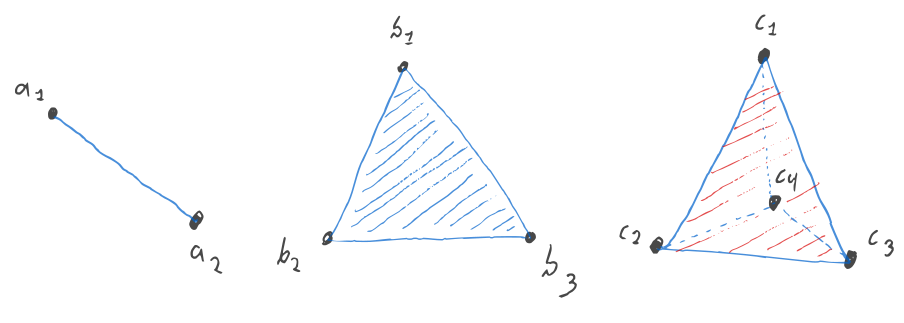
\includegraphics[width=0.8\textwidth]{png/Eksempel1-8.png}
			%\includesvg[width=0.6\textwidth]{Eksempel1-8.svg}
			\caption{Tre geometriske simpleksar.}
			\label{fig:tre-geometriske-simpleksar}
		\end{center}
	\end{figure}
\end{example}

\begin{remark}
	Noko som er svært interessant med denne definisjonen er at om ein har ei geometrisk uavhengig mengd $P$, og ser på $\hat{P}_i := P \setminus \{p_i\}$, så vil dette også vera ei geometrisk uavhengig mengd. I tillegg så vil det geometriske simplekset utspent av $\hat{P}_i$ vera ei delmengd av det geometriske simplekset utspent av $P$. Med andre ord, alle delmengder av $P$ dannar også geometriske simpleks, inneheldt i det originale geometriske simplekset! Men ikkje nok med det! Når ein ser på det geometriske simplekset utspent av $\hat{P}_i$ for ein eller annan $i$, så ser ein at det er som eine "<fjeset"> av det geometriske simplekset utspent av $P$. Om ein vidare ser på unionen av alle geometriske simpleks utspent av \( \hat{P}_i \) for alle \( i \), så gir dette randen til det geometriske simplekset utspent av \( P \). Dette kan ein sjå i \autoref{fig:tre-geometriske-simpleksar}, der den geometriske simpleksen utspent av \( \set{b_1, b_2} \), er eine "<fjeset"> til det geometriske simplekset utspent av \( \set{b_1, b_2, b_3} \), og unionen av ale dese fjesa vil vera heile randen til det geometriske simplekset utspent av \( \set{b_1, b_2, b_3} \).
\end{remark}

\begin{definition}
	La $V$ vera ei endeleg mengd, og $f:V\rightarrow \Rb^m$ ei injektiv avbilding der bilete $f(V)$ er ei geometrisk uavhengig mengd av punkt. 
	
	Då kallar me \( f \) for ei \emph{affin imbedding}.
\end{definition}

\begin{definition} \label{def:gr}
	La \( K \) vera eit endeleg abstrakt simplisielt kompleks $K$ over ei ikkje-tom hjørnemengd $V$, og la $f:V\to\Rb^m$ vera ei affin imbedding.
	
	Då er den \emph{geometriske realiseringa med omsyn på $f$ av \( K \)}, unionen av alle dei geometriske simpleksa utspent av punkta i $f(\sigma)$, for alle $\sigma\in K$. Dette er ofte skrive $\gr{K}_f$.
\end{definition}

\begin{remark} \label{rem:gr-SK}
	Det er ofte at ein brukar same notasjon når ein tenker på eit geometrisk simpleks med (geometrisk uavhengig) hjørnemengd \( \set{f(v_1), f(v_2), \dots, f(v_n)} \) for eit abstrakt \( (n-1) \) simpleks \( V := \set{v_1, v_2, \dots, v_n} \). Ein skriv dette som \( \gr{V}_f \), der ein tenker at ein tek den geometriske realiseringa over det minste abstrakte simplisielle komplekset som inneheld \( V \). Altså \( \gr{V}_f := \gr{\set{\tau : \tau \subseteq V}}_f \).
\end{remark}

\begin{lemma} \label{thm:tau-homeomorfi}
	La \( K \) vera eit abstrakt simplisielt kompleks over \( V \), og la \( f: V \to \Rb^n \) vera ei affin imbedding. Fiksér ein vilkårleg \( x \in \Rb^n \).
	
	La
	\begin{align*}
		\tau: \Rb^n &\to \Rb^n \\
		y &\mapsto y - x
	\end{align*}
	og la
	\begin{align*}
		\hat{\tau} := \tau|_{\gr{K}_f}: \gr{K}_f &\to \gr{K}_{\hat{\tau} \circ f} \\
		y  &\mapsto y - x.
	\end{align*}

	Då er \( \hat{\tau} \) veldefinert og ein homeomorfi, og \( \hat{\tau} \circ f \) er ei affin imbedding.
\end{lemma}

\begin{proof}
	For å visa at \( \hat{\tau} \circ f \) er ei affin imbedding, så ser ein på \( \hat{\tau} \circ f(V) = (f(v_1)-x, f(v_2)-x, \dots, f(v_n)-x) \). Ein får då at 
	\begin{align*}
		(f(v_2)-x-(f(v_1)-x), &f(v_3)-x-(f(v_1)-x), \dots, f(v_n)-x-(f(v_1)-x)) = \\
		&( f(v_2)-f(v_1), f(v_3)-f(v_1), \dots, f(v_n)-f(v_1) ) .
	\end{align*}

	Frå \autoref{thm:geometrisklineærtuavhengig}, får ein at \( ( f(v_2)-f(v_1), f(v_3)-f(v_1), \dots, f(v_n)-f(v_1) ) \) er lineært uavhengig fordi \( f(V) \) er geometrisk uavhengig. Det tyder igjen at \( (f(v_2)-x-(f(v_1)-x), f(v_3)-x-(f(v_1)-x), \dots, f(v_n)-x-(f(v_1)-x)) \) er lineært uavhengig, som tyder at \( \hat{\tau} \circ f(V) \) er geometrisk uavhengig.

	For å visa at \( \hat{\tau}(\gr{K}_f) \subseteq \gr{K}_{\hat{\tau} \circ f} \), så ser ein på \( y \in \hat{\tau}(\gr{K}_f) \). Då er \( y \) ein konveks kombinasjon av \( f(\sigma) \) for ein eller annan \( \sigma \in K \). Det vil seie at for \( k \) lik talet på element i \( f(\sigma) \), så er \( y = \sum_{i=1}^k a_i f(v_i) \). Då er
	\begin{align*}
		\hat{\tau}(y) &= \left(\sum_{i=1}^k a_i f(v_i)\right) - x \\
		&= \left(\sum_{i=1}^k a_i f(v_i)\right)-\left(\sum_{i=1}^k a_i \right)x 
		\tag{Hugs at \( \sum_{i=1}^k a_i = 1 \)} \\
		&= \left(\sum_{i=1}^k a_i f(v_i)\right)-\sum_{i=1}^k a_i x \\
		&= \sum_{i=1}^k \tuple{a_i f(v_i) - a_i x} \\
		&= \sum_{i=1}^k a_i(f(v_i) - x)
	\end{align*}
	som er ein konveks kombinasjon av element i \( \hat{\tau} \circ f(\sigma) \), og difor ei delmengd av \( \gr{K}_{\hat{\tau} \circ f} \).

	For å visa at \( \hat{\tau}(\gr{K}_f) \supseteq \gr{K}_{\hat{\tau} \circ f} \), så lar ein \( y \in \gr{K}_{\hat{\tau} \circ f} \). For ein eller annan \( \sigma \in K \) får ein då at \( y \) er ein konveks kombinasjon av element i \( \hat{\tau}\circ f(\sigma) \). Altså: \(  y = \sum_{i=1}^k a_i (f(v_i) - x) \). Ein lik sum-manipulasjon som ovanfor, berre motsett veg, gir ein at \( y = \hat{\tau}\left(\sum_{i=1}^k a_i f(v_i)\right) \), altså \( \hat{\tau}(z) \), der \( z \) er ein konveks kombinasjon av punkta \( f(\sigma) \). Altså \( y \) er eit element i \( \hat{\tau}(\gr{K}_f) \).

	Merk at \( \hat{\tau} = \tau \circ i \), der \( \tau: \Rb^n \to \Rb^n \) er ein homeomorfi og \( i: \gr{K}_f \hookrightarrow \Rb^n \) er inklusjonen inn i \( \Rb^n \). \autoref{thm:universal-eigenskap-underromstopologi} gir då at \( \hat{\tau} \) er kontinueleg.

	Ved symmetri så kan ein gjera eit likt argument på \( \hat{\tau}^{-1}: y \mapsto y+x \), og ein får difor at \( \hat{\tau} \) er ein homeomorfi.
\end{proof}

\begin{theorem} \label{thm:gr-eintydig}
	Geometrisk realisering er eintydig opp til homeomorfi. Med andre ord: For to ulike geometriske realiseringar av eit endeleg abstrakt simplisielt kompleks $K$, med omsyn på $f$ og $g$ (to ulike affine imbeddingar), så er $\gr{K}_f$ og $\gr{K}_g$ homeomorfe.
\end{theorem}

\begin{proof}
	La $K$ vera eit abstrakt simplisielt kompleks, og la $V=\{ v_1, v_2, \dots, v_n \}$ vera hjørnemengda til $K$. La $f:V\to\Rb^m$ og $g:V\to\Rb^l$ vera to affine imbeddingar. Definér vidare $x_i=(f(v_{i-1})-f(v_1))$ og $y_i=(g(v_{i-1})-g(v_1))$. La $\tau_f:\Rb^m\to\Rb^m$ vera ei forskyving som tek $x\mapsto x-f(v_1)$, og la $\tau_g:\Rb^l\to\Rb^l$ vera ein forskyving som tek $x\mapsto x-g(v_1)$. Til slutt, Definér $\hat{f}:=\tau_f\circ f$ og $\hat{g}:=\tau_g \circ g$.
	
	la $L_1:\Rb^m\to\Rb^l$ vera ei lineær funksjon som sender $x_i\mapsto y_i$. Det er mogleg sidan \( \set{x_i}_{i=2}^{\#V} \) er ei lineært uavhengig mengd frå \autoref{thm:geometrisklineærtuavhengig}, så ein kan bruka \autoref{thm:definer-lin-op} på dei, og \( x_1 \mapsto y_1 \) følger ettersom \( x_1 = 0 \mapsto 0 = y_1 \).

	Ein får då at $L_1(\hat{f}(v_i))=\hat{g}(v_i)$, fordi:
	
	For $i=1$, så er

	\[
		L_1(\hat{f}(v_1))=L_1(f(v_1)-f(v_1))=L(0)=0=g(v_1)-g(v_1)=\hat{g}(v_1).
	\]

	For $i\neq 1$, så er

	\[
		L_1(\hat{f}(v_i))=L_1(f(v_i)-f(v_1))=L_1(x_{i-1})=y_{i-1}=g(v_i)-g(v_1)=\hat{g}(v_i).
	\]

	Om ein då lar $L_2:\Rb^l\to\Rb^m$ vera den lineære funskjonen som sender $y_i\mapsto x_i$, så er definisjonane symmetriske og \( L_2(\hat{g}(v_i))=\hat{f}(v_i) \) frå det same argumentet som ovanfor.

	La $\hat{L} := L_1|_{\gr{K}_{\hat{f}}}$, og $\tilde{L} := L_2|_{\gr{K}_{\hat{g}}}$.

	For eit vilkårleg element $x\in\gr{K}_{\hat{f}}$ så kan ein kan utrykka $x$ som ein konveks kombinasjon av ei geometrisk uavhengig mengd som korresponderer til hjørnemengda \( \hat{f}(\sigma) = \{\hat{f}(v_1), \hat{f}(v_2), \dots, \hat{f}(v_k)\} \) for ein eller annan \( \sigma \in K \).
	
	Då er $x=\sum_{i=1}^ka_i\hat{f}(v_i)$ med $\sum_{i=1}^ka_i=1$ og $a_i\geq0\; \forall i$. 
	
	Her er valet av kva hjørnemengd ein ser \( x \) som ein konveks kombinasjon over ikkje viktig, ettersom $\hat{L}$ er veldefinert.
	\begin{align*}
		\tilde{L}\circ \hat{L}(x) &= \tilde{L}\circ \hat{L}\left(\sum_{i=1}^ka_i\hat{f}(v_i)\right) \\
		&= \tilde{L}\left(\sum_{i=1}^k\hat{L}(a_i\hat{f}(v_i))\right) \\
		&= \tilde{L}\left(\sum_{i=1}^ka_i\hat{L}(\hat{f}(v_i))\right) \\
		&= \tilde{L}\left(\sum_{i=1}^ka_i\hat{g}(v_i)\right) \\
		\intertext{ettersom $\sum_{i=1}^ka_i\hat{g}(v_i)\in\gr{K}_{\hat{g}}$, så får ein at} \\
		\tilde{L}\left(\sum_{i=1}^ka_i\hat{g}(v_i)\right) &= \sum_{i=1}^k\tilde{L}(a_i\hat{g}(v_i)) \\
		&= \sum_{i=1}^ka_i\tilde{L}(\hat{g}(v_i)) \\
		&= \sum_{i=1}^ka_i\hat{f}(v_i) \\
		&= x.
	\end{align*}
	Ein kan gjere det same for $\hat{L}\circ\tilde{L}(y)$ ved eit symmetrisk argument. Dette tyder at $\hat{L}$ er bijektiv med invers $\tilde{L}$.
	
	Om ein lar $\hat{\tau}_f:=\tau_f|_{\gr{K}_f} : \gr{K}_f \to \gr{K}_{\hat{f}}$ og $\hat{\tau}_g:=\tau_g|_{\gr{K}_g} : \gr{K}_g \to \gr{K}_{\hat{g}}$, så får ein frå \autoref{thm:tau-homeomorfi} at desse er homeomorfiar.
	
	Då får ein det følgande kommutative diagrammet:
%	\begin{center}
%		\begin{tikzpicture}
%			\diagram{d}{2.5em}{2.5em}{
%				\Rb^m & \Rb^m & \Rb^l & \Rb^l \\
%				\vert K\vert_f & \vert K\vert_{\hat{f}} & \vert K\vert_{\hat{g}} & \vert K\vert_g \\
%				};
%		\path[->,font = \scriptsize, midway]
%		(d-1-1) edge node[above]{$\tau_f$} (d-1-2)
%		(d-1-2) edge node[above]{$L$} (d-1-3)
%		(d-1-4) edge node[above]{$\tau_g$} (d-1-3)
%		(d-2-1) edge [dashed,->] node[below]{$\hat{\tau}_f$}(d-2-2)
%		(d-2-2) edge node[below]{$\hat{L}$} (d-2-3)
%		(d-2-4) edge [dashed,->] node[below]{$\hat{\tau}_g$} (d-2-3)
%		(d-2-1) edge (d-1-1)
%		(d-2-2) edge (d-1-2)
%		(d-2-3) edge (d-1-3)
%		(d-2-4) edge (d-1-4);
%		\end{tikzpicture}
%	\end{center}
	\begin{center} % |, \vert funke ikkje??
		\begin{tikzcd}
			\Rb^m \arrow{r}{\tau_f}
			& \Rb^m \arrow{r}{L}
			& \Rb^l
			& \Rb^l \arrow{l}[swap]{\tau_g} \\
			\gr{K}_f \arrow[dashed]{r}{\hat{\tau}_f} \arrow[hook]{u}
			& \gr{K}_{\hat{f}} \arrow{r}{\hat{L}} \arrow[hook]{u}
			& \gr{K}_{\hat{g}} \arrow[hook]{u}
			& \gr{K}_g \arrow[dashed]{l}[swap]{\hat{\tau}_g} \arrow[hook]{u}
		\end{tikzcd}
	\end{center}
	der alle dei vertikale avbildingene er dei naturlege inklusjonane.

	Merk her at avbildinga \( \hat{L} \) på nedste rad er kontinuerleg ifølge \autoref{thm:universal-eigenskap-underromstopologi}. I tillegg så har ein at \( \hat{\tau}_f \) og \( \hat{\tau}_g \) er homeomorfiar.

	Sidan $\hat{L}$ er både kontinuerleg og bijektiv, med invers $\tilde{L}$ som frå eit symmetrisk argument også er kontinuerleg. Så har ein at $\hat{L}$ er ein homeomorfi.

	Ein får at avbildinga $(\hat{\tau}_g)^{-1}\circ\hat{L}\circ\hat{\tau}_f:\gr{K}_f\to\gr{K}_g$ er ei samansetting av tre homeomorfiar, og er difor ein homeomorfi sjølv.
\end{proof}

\begin{remark}
	Ettersom alle forskjellige geometriske realiseringar er homeomorfe grunna det førre resultatet, så er det vanleg å snakka om \emph{den} geometriske realiseringa av eit abstrakt simplisielt kompleks $K$. Difor plar ein å sløyfa subskrifta i notasjonen og berre bruka $\gr{K}$ for \emph{den} geometriske realiseringa av $K$.
\end{remark}

\begin{definition} \label{def:cech}
	La \( P \) vera ei endeleg mengd av punkt i \( \Rb^m \), og la \( r \in [0, \infty) \).
	
	Då er \emph{Cech-komplekset til $P$ med radius $r$} definert som
	\[
		\Cech_r(P) := \left\{\sigma\subseteq P : \intersect_{p\in\sigma}\bar{B}_r(p)\neq\emptyset\right\}.
	\]
\end{definition}

\begin{example}
	 I \autoref{fig:tre-cech-kompleks} så kan ein sjå tre ulike døme på korleis Cech-komplekset ser ut med varierande radius. Merk her at det skal vera ballar med same radius i kvart døme, men det var vanskeleg å teikna.
	\begin{figure}[htbp]
		\begin{center}
			\includesvg[width=0.8\textwidth]{Eksempel1_18-2.svg}
		\end{center}
		\caption{Tre døme på Cech-kompleks.}
		\label{fig:tre-cech-kompleks}
	\end{figure}
\end{example}

\begin{theorem} \label{thm:CASK}
	La \( P \) vera ei endeleg mengd av punkt i \( \Rb^m \) med \( r \in [0, \infty) \).
	
	Då er Cech-komplekset til $P$ med radius $r$ eit abstrakt simplisielt kompleks over $P$.
\end{theorem}

\begin{proof}
	For å visa dette, så må ein visa at alle dei tre aksioma i \autoref{def:ASK} held:
	\begin{enumerate}
		\item{ For ein \( \hat{p} \in P \) så ser ein at for \( \sigma = \set{\hat{p}} \), så er \( \intersect_{p\in\sigma}\bar{B}_r(p)=\bar{B}_r(\hat{p})\neq\emptyset \) og då er \( \set{\hat{p}} \in \Cech_r(P) \). }
		\item{ Per definisjon av Cech-komplekset, så er alle \( \sigma \in \Cech_r(P) \) ei delmengd av \( P \). }
		\item{ For \( \sigma \in \Cech_r(P) \), så ser ein at \( \intersect_{p\in\sigma} \bar{B}_r(p) \neq \emptyset \). Men det tyder at for alle \( \tau \subseteq \sigma \), så er \( \intersect_{p\in\tau} \bar{B}_r(p) \) også ikkje-tom, for om den var tom, så ville
			\[ 
				\intersect_{p\in\sigma} \bar{B}_r(p) = \left( \intersect_{p\in(\sigma\setminus\tau)} \bar{B}_r(p) \right) \intersect \left( \intersect_{p\in\tau} \bar{B}_r(p) \right) = \left( \intersect_{p\in(\sigma\setminus\tau)} \bar{B}_r(p) \right) \intersect \emptyset = \emptyset 
			\] 
			som ikkje er sant. Difor må \( \tau \in \Cech_r(P) \). }
	\end{enumerate}
\end{proof}

Eit fint resultat som er ekvivalent med definisjonen av Cech-komplekset er som følger:

\begin{theorem}
	La $P$ vera ei endeleg mengd av punkt i $\Rb^m$ og la $r\in[0, \infty)$.

	Då er \( \sigma \in \Cech_r(P) \) visst og berre visst det eksisterer ein \( x \in \Rb^m \) sånn at \( \sigma \subseteq \bar{B}_r(x) \).
\end{theorem}

\begin{proof}
	($\implies$)
	
	Sidan $A:=\intersect_{p\in\sigma}\bar{B}_r(p)\neq\emptyset$, så finst det ein $x\in A$ der for for alle \( p\in\sigma \) så er \( d(p,x)\leq r \), sidan $x\in\bar{B}_r(p)$.
	
	Men sidan $d(p,x)=d(x,p)$ per definisjon av metrikk, så får ein at \( \forall p\in\sigma \) så er \( p \in \bar{B}_r(x) \).
	
	( \( \Longleftarrow \) )
	
	Ved eit likt argument så ser ein at om alle \( p \in \sigma \) gir at \( d(x, p) \leq r \) så betyr det at \( d(p, x) \leq r \) for alle \( p \in \sigma \). Men det betyr at \( x \in \intersect_{p \in \sigma} \bar{B}_r(p) \), som igjen betyr at \( \intersect_{p \in \sigma} \bar{B}_r(p) \neq \emptyset \).
\end{proof}

Arbeidet fram til no gir ein nok grunnlag til å endeleg kunne forstå og definera nerva, som er ein sentral del av nerveteoremet:

\begin{definition} \label{def:nerva}
	La $X$ vera eit ikkje-tomt topologisk rom. Vidare la $F$ vera ei mengd av underrom av $X$. 
	
	Definér \emph{nerva til $F$}, skrive $\Nc(F)$, som
	\begin{equation*}
		\Nc(F) := \left \{ \sigma \subseteq F : \intersect_{ F_i \in \sigma } F_i \neq \emptyset \right \}
	\end{equation*}
\end{definition}

\begin{theorem}
	La $X$ vera eit topologisk ikkje-tomt topologisk rom, og la $F$ vera ei mengd av underrom av $X$.
	
	Då er nerva til $F$ eit abstrakt simplisielt kompleks over $F$.
\end{theorem}

\begin{proof}
	Som i beviset for at Cech-komplekset er eit abstrakt simplisielt kompleks (\autoref{thm:CASK}), så må ein visa at alle krava i \autoref{def:ASK} er oppfylte:
	\begin{enumerate}
		\item{ 
			For \( v \in F \) har ein at for \( \sigma = \set{ v } \) så er \( \intersect_{ p \in \sigma } p = v \neq \emptyset \), så \( \set{v} \in \Nc(F) \).
		}
		\item{ 
			Alle element i \( \Nc(F) \) er per definisjon ei delmengd av \( F \).
		}
		\item{  
			For \( \sigma \in \Nc(F) \) ser ein at \( \intersect_{v\in\sigma} v \neq \emptyset \). Det tyder at for alle \( \tau \subseteq \sigma \), så er \( \intersect_{v\in\tau} v \) også ikkje-tom, for om \( \intersect_{v\in\tau} v = \emptyset \), så ville 
			\[ 
				\intersect_{v\in\sigma} v = \left( \intersect_{v\in(\sigma\setminus\tau)} v \right) \intersect \left( \intersect_{v\in\tau} v \right) = \left( \intersect_{v\in(\sigma\setminus\tau)} v \right) \intersect \emptyset = \emptyset 
			\] 
			som ikkje er sant. Difor må \( \tau \in \Nc(F) \).
		}
	\end{enumerate}
\end{proof}

\begin{example}
	I \autoref{fig:tre-gr} kan ein sjå tre døme på mengder av delmengder i \( \Rb^2 \) og den geometriske realiseringa av nerva deira.
	\begin{figure}[htbp]
		\begin{center}
			\includesvg[width=0.6\textwidth]{Eksempel1_23.svg}
		\end{center}
		\caption{Tre døme på geometrisk realisering.}
		\label{fig:tre-gr}
	\end{figure}
\end{example}

\begin{remark} \label{rem:cech-ekvivalent}
	Direkte frå \autoref{def:nerva} så ser ein at Cech-komplekset til $P$ med radius $r$ (som gitt i \autoref{def:cech}), er "<ekvivalent"> til nerva til $\union_{p \in P} \left \{ \bar{B}_r(p) \right \}$. Meir om kva "<ekvivalent"> tyder i denne samanhengen kjem seinare i teksten.
\end{remark}

Då kan ein endeleg utrykka nerveteoremet:

\begin{theorem}[Nerveteoremet] \label{thm:nerveteoremet}
	La \( \Rb^d \) ha standardtopologien, og la \( U = \set{U_i}_{i=1}^n \) vera ei endeleg mengd av kompakte og konvekse delmengder av \( \Rb^d \) med underromstopologien.
	
	Då er \( \union_{u \in U} u \) homotopiekvivalent med \( \gr{\Nc(U)} \).
\end{theorem}

Merk at dette er kun eit av mange ulike nervetorem som eksisterer, som nemd i \autoref{sec:innleiing}, men dei har mange ting til felles. Alle seier at ein kan kondensera all "<strukturen"> til eit topologisk rom opp til homotopiekvivalens inn i eit abstrakt simplisiellt kompleks om ein finn eit riktig overdekke av det. Dette er det som gjer nerveteorema så sterke.

Nerveteoremet i det kompakte og konvekse tilfellet som eg skriv om, er det som blir vanlegast brukt i topologisk dataanalyse, ettersom det er det ein får mest bruk for.

Den mest vanlege anvendinga av nerveteoremet i topologisk dataanalyse er å sjå på Cech-komplekset. Sidan Cech-komplekset er "<ekvivalent"> til nerva til \( \union_{p \in P} \left \{ \bar{B}_r(p) \right \} \), og sidan \( \bar{B}_r(p) \) er kompakt og konveks, så fungerer nerveteoremet for det. Det viser at Cech-komplekset bevarer nesten heile den topologiske strukturen til \( \union_{p \in P} \bar{B}_r(p) \).

Dette er veldig praktisk, ettersom Cech-komplekset er ein svært naturleg ting ein vil sjå på om ein er ute etter "<strukturen"> til ei datamengd.

I neste seksjon så kjem eit bevis av dette nerveteoremet.

\section{Bevis for nerveteoremet}

Dette beviset er svært inspirert av \cite[Section 3]{https://doi.org/10.48550/arxiv.2203.03571}.

\begin{definition}
	La \( K \) vera eit endeleg abstrakt simplisielt kompleks over \( V \). 
	
	Då er den \emph{barysentriske oppdelinga} av \( K \), skriven \( \Sd(K) \), alle tuplar på forma: 
	\[
		\set{(\sigma_1, \sigma_2, \sigma_3, \dots, \sigma_n) \mid \sigma_1 \subsetneq \sigma_2 \subsetneq \sigma_3 \subsetneq \dots \subsetneq \sigma_n\,, \sigma_i \in K}.
	\]
\end{definition}

\begin{lemma} \label{thm:subdivisjon-abstrakt-simplisielt-kompleks}
	La \( K \) vera eit endeleg abstrakt simplisielt kompleks over \( V \).
	
	Då er \( \Sd(K) \) eit endeleg abstrakt simplisielt kompleks over \( K \).
\end{lemma}

\begin{proof}
	Ein må visa at dei tre krava i \autoref{def:ASK}:
	\begin{enumerate}
		\item{ For \( k \in K \), så er \( \tuple{k} \) trivielt ei streng følge av element i \( K \), så \( \tuple{k} \in \Sd(K) \). }
  		\item{ For \( \sigma \in \Sd(K) \) så er \( \sigma \) per definisjon ei delmengd av \( K \). }
    	\item{ For \( \sigma \in K \), med \( \tau \subseteq \sigma \), så er \( \tau \) ei delfølge av element frå \( K \). Men ei delfølge er framleis ei følge, så \( \tau \in \Sd(K) \). }
	\end{enumerate}
\end{proof}

\begin{remark}
	Grunnen til at ein kallar den barysentriske oppdelinga til \( K \) for \( \Sd(K) \), er at den barysentriske oppdelinga av eit abstrakt simplisielt kompleks ofte kalla for ein "<subdivision"> på engelsk.
\end{remark}

\begin{lemma} \label{thm:geometrisk-kompleks-lukka}
	La \( K \) vera eit endeleg abstrakt simplisielt kompleks over \( V \) og la \( f: V \to \Rb^d \) vera ei affin imbedding.
	
	Då er \( \gr{K}_f \) lukka og kompakt.
\end{lemma}

\begin{proof}
	Ein ser på eit vilkårleg geometrisk \( n \)-simpleks i \( \Rb^n \) med hjørne i \( \tuple{0, e_1, e_2, \dots, e_n} \), der \( \tuple{e_1, e_2, \dots, e_n} \) er standardbasisen til \( \Rb^n \). Dette er ei geometrisk uavhengig mengd ifølge \autoref{thm:geometrisklineærtuavhengig} sidan \( \tuple{e_1, e_2, \dots, e_n} \) er lineært uavhengig per definisjon. Ein kallar denne \( n \)-simpleksen for \( \Delta^n \).

	La \( U_i \) vera hyperplanet definert av å gå gjønom dei \( n \) punkta \( \tuple{0, e_1, \dots, e_{i-1}, e_{i+1}, \dots, e_n} \), og så ser ein på halvplanet danna av den delen av \( \Rb^n \setminus U_i \) som ikkje inneheld \( e_i \) (For \( i=1 \), så ser ein på planet der ein fjernar punktet \( 0 \).). Dette kallar ein for \( \hat{U}_i \). Dette er ei open mengda i \( \Rb^n \), sidan det er ein homeomorfi frå \( \Rb^n \) til \( \Rb^n \), som sender \( \hat{U}_i \) til det standard øvre hyperplanet \( H^n := (0, \infty) \times \Rb^{n-1} \).

	La \( x \in \Rb^n \). Då kan ein skriva \( x \) som ein unik lineærkombinasjon av standardbasisen, altså \( x = \sum_{i=1}^n a_ie_i \). 

	Ein har at for \( j \neq 0 \), så er \( \hat{U}_j \), hyperhalvplanet danna av den sida av \( U_j \) som ikkje inneheld \( e_j \). Men sidan \( U_j \) er hyperhalvplanet danna av alle punkt der den \( j \)-te koordinaten er \( 0 \), og sidan \( e_j \) har opplagt positiv \( j \)-te koordinat, så då er \( \hat{U}_j = \Rb^{j-1}\times(-\infty, 0) \times \Rb^{n-j} \).

	For \( j = 0 \), så er \( \hat{U}_0 \), hyperhalvplanet dana av sida av \( U_0 \) som ikkje inneheld \( 0 \). Men sidan \( U_0 \) er hyperhalvplanet danna av alle \( x \in \Rb^n \),  der \( x = \sum_{i = 1}^n a_i e_i \), med \( \sum_{i = 1}^n a_i = 1 \), og sidan \( x = 0 \), så er \( a_i = 0 \) for alle \( i \). Difor må \( \hat{U}_0 \) vera hyperhalvplanet som består av alle \( x = \sum_{i = 1}^n a_i e_i \) der \( \sum_{i = 1}^n a_i > 1 \).

	Merk at \( x \in \Delta^n \) visst og berre visst \( \sum_{i=1}^n a_i \leq 1 \) og \( a_i \geq 0 \) for alle \( i = 1, 2, \dots, n \), sidan ein kan alltid definere \( a_0 = 1 - \sum_{i=1}^n a_i \geq 0 \), utan å endre koordinat.

	For \( x \not\in \Delta^n \) då er det to ulike tilfeller som kan skje:

	\begin{enumerate}
		\item { Ein kan ha at \( a_j < 0 \) for ein eller annan \( j \neq 0 \).
		
				Men då er \( x \in \hat{U}_j \), sidan \( \hat{U}_j = \Rb^{j-1}\times(-\infty, 0) \times \Rb^{n-j} \). }
  		\item { Eller ein kan ha at alle \( a_j \geq 0 \), men \( \sum_{i=1}^n a_i > 1 \). 
		
				 Då er \( x \in \hat{U}_0 \), fordi \( \hat{U}_0 \) er hyperhalvplanet som består av alle \( x = \sum_{i = 1}^n a_i e_i \) der \( \sum_{i = 1}^n a_i > 1 \). }
	\end{enumerate}

	Difor så får ein at for \( x \not\in \Delta^n \) så er \( x \in \hat{U} \).

	For \( x \in \Delta^n \), så er \( x = \sum_{i=1} a_i e_i \), med \( a_i \geq 0 \), og \( \sum_{i=1}^n a_i \leq 1 \).

	Då er det opplagt at \( x \not\in \hat{U}_j \) for \( j \neq 0 \), sidan den \( j \)-te koordinaten ikkje er strengt negativ og \( \hat{U}_j = \Rb^{j-1}\times(-\infty, 0) \times \Rb^{n-j} \). I tillegg, så er det opplagt at \( x \not\in \hat{U}_0 \), sidan \( \hat{U}_0 \) er hyperhalvplanet som består av alle \( x = \sum_{i = 1}^n a_i e_i \) der \( \sum_{i = 1}^n a_i > 1 \).

	Så ein får at for \( x \in \Delta^n \) så er \( x \not\in \hat{U} \).

	Samlar ein saman dei to resultata, får ein at \( \Rb^n \setminus \hat{U} = \Delta^n \). Og sidan \( \hat{U} \) er ein union av opne mengder, så er \( \hat{U} \) open. Det gir ein at \( \Delta^n \) er lukka.

	Vidare, sidan alle hjørna til \( \Delta^n \) er inne i den lukka ballen \( \bar{B}_{1}(0) \), som er konveks, så seier \autoref{thm:konveks-kombinasjon-i-konveks} at \( \Delta^n \in \bar{B}_{1}(0) \). Det gir at \( \Delta^n \) er både avgrensa og lukka. \autoref{thm:heine-borel} gir ein difor at \( \Delta^n \) er kompakt.

	Gitt eit vilkårleg geometrisk \( n \)-simpleks i \( \Rb^d \) kalla for \( \hat{\Delta}^n \), sjå på avbildinga \( \Delta^n \to \hat{\Delta}^n \) som blir danna i \autoref{thm:gr-eintydig} om ein tenker på \( \Delta \) og \( \hat{\Delta} \) som geomeriske realiseringar av det minimale abstrakte simpliselle komplekset som inneheld \( \set{v_1, v_2, \dots, v_n} \), som i \autoref{rem:gr-SK}. Sidan denne avbildninga er ein homeomorfi og \( \Delta^n \) er kompakt, så er \( \hat{\Delta}^n \) også kompakt.

	\autoref{thm:heine-borel} gir ein då at \( \hat{\Delta}^n \) er både lukka og kompakt i \( \Rb^d \).

	Og sidan ei vilkårleg geometrisk realisering er ein union av endeleg mange geometriske simpleksar, så er det ein endeleg union av lukka og kompakte mengder, og difor ei lukka og kompakt mengd sjølv ifølge \autoref{thm:endeleg-union-kompakt-er-kompakt}.
\end{proof}

\begin{lemma} \label{thm:alpha-homeomorfi}
	La \( K \) vera eit endeleg abstrakt simplisielt kompleks over \( V \), la \( f: \Nc(U) \to \Rb^d \) vera ei affin imbedding, og la \( g: U \to \Rb^m \) vera ei affin imbedding.
	
	Då er \( \gr{\Sd(K)}_f  \) homeomorf med \( \gr{K}_g \) ved ein homeomorfi ein kallar for \( \alpha \) som vert definert i slutten av beviset nedanfor.
\end{lemma}

\begin{proof}
	Dette beviset brukar mykje den same strategien som i \autoref{thm:gr-eintydig}.

	Fyrst, lag ei ordning av elementa i \( V = (v_1, v_2, \dots, v_n) \) og ei ordning \( K = (\sigma_1, \sigma_2, \dots, \sigma_m) \) med \( \sigma_1 = \set{v_1} \). Vidare la \( \tau_f(x) := x-f(\set{v_1}) \), og la \( \tau_g(x) := x-g(v_1) \). Desse er homeomorfiar frå \autoref{thm:tau-homeomorfi}.

	Definer \( \hat{f} := \tau_f \circ f \) og \( \hat{g} := \tau_g \circ g \).

	Då kan ein definera ein lineæroperator \( L: \Rb^d \to \Rb^m \) definert for \( \sigma \in K \) ved å senda \( \hat{f}(\sigma) \mapsto \frac{1}{\#\sigma}\sum_{v_j \in \sigma} \hat{g}(v_j) \). Dette er mogleg fordi \( \hat{f}(K) = (0, f(\sigma_2)-f(\sigma_1), f(\sigma_3)-f(\sigma_1), \dots, f(\sigma_n)-f(\sigma_1) ) \), er lineært uavhengige sidan \( f \) er ei affin imbedding, og \autoref{thm:geometrisklineærtuavhengig} (utanom \( 0 \), som blir sendt til \( 0 \) uansett frå linearitet), så \autoref{thm:definer-lin-op} gjeld.

	Ein veit då frå \autoref{thm:avgrensa-lin-op-er-kont} at \( L \) er kontinuerleg. 

	Vidare så får ein at \( L(\gr{\Sd(K)}_{\hat{f}}) \subseteq \gr{K}_{\hat{g}} \). Sidan for \( x \in \gr{\Sd(K)}_{\hat{f}} \), så er \( x \) ein konveks kombinasjon av punkt \( \hat{f}(\sigma) \) for ein eller annan \( \sigma \in \Sd(K) \), frå definisjonen av geometrisk realisering (\autoref{def:gr}). La \( \sigma = (\sigma_1, \sigma_2, \dots, \sigma_{\#\sigma}) \). Då er \( x = \sum_{i=1}^{\#\sigma} a_i \hat{f}(\sigma_i) \), med \( (a_i)_i^{\#\sigma} \) dei barysentriske koordinatane til \( x \). Ein får då
	\begin{align*}
		L(x) &= L\left(\sum_{i=1}^{\#\sigma} a_i \hat{f}(\sigma_i)\right) \\
		&= \sum_{i=1}^{\#\sigma} L(a_i \hat{f}(\sigma_i)) \\
		&= \sum_{i=1}^{\#\sigma} a_i L(\hat{f}(\sigma_i)) \\
		&= \sum_{i=1}^{\#\sigma} a_i \frac{1}{\#\sigma_i} \sum_{v_j \in \sigma_i} \hat{g}(v_j) \\
		&= \sum_{i=1}^{\#\sigma} \sum_{v_j \in \sigma_i} a_i \frac{1}{\#\sigma_i} \hat{g}(v_j).
	\end{align*}
	Summen av koeffisientane til \( \hat{g}(v_j) \)-ane er difor
	\[
		\sum_{i=1}^{\#\sigma} \sum_{v_j \in \sigma_i} a_i \frac{1}{\#\sigma_i} = 
		\sum_{i=1}^{\#\sigma} \#\sigma_i a_i \frac{1}{\#\sigma_i} =
		\sum_{i=1}^{\#\sigma} a_i = 1
	\]
	og sidan for ein \( \sigma \in \Sd(K) \) så er \( \union_{\sigma_i \in \sigma} \sigma_i = \sigma_{\#\sigma} \in K \). Då er \( x \) i eit geometrisk simpleks utspent av punkta \( \hat{g}(\sigma_{\#\sigma}) \), men sidan \( \sigma_i \in \Nc(U) \) for alle \( i \), så må \( \sigma_{\#\sigma} \in \Nc(U) \) som gir at \( x \in \gr{\sigma_{\#\sigma}}_{\hat{g}} \subseteq \gr{K}_{\hat{g}} \).

	Definér \( \hat{L} := L|_{\gr{\Sd(K)}_{\hat{f}}}: \gr{\Sd(K)}_{\hat{f}} \to \gr{K}_{\hat{g}} \).

	Frå den universale eigenskapen av underromstopologien (\autoref{thm:universal-eigenskap-underromstopologi}) så får ein at \( \hat{L} \) er kontinuerleg.

	Vidare, definer avbildinga \( \tilde{L} \) punktvis:
	
	For ein \( y \in \gr{K}_{\hat{g}} \), så er \( y \) ein konveks kombinasjon av punkt \( \hat{g}(\epsilon) \) for ein \( \epsilon \in K \), med barysentriske koordinatar \( \tuple{b_1, b_2, b_3, \dots, b_{\#\epsilon}} \). Vel ei ordning av \( \epsilon = \tuple{v_1, v_2, \dots, v_{\#\epsilon}} \) sånn at \( b_1 \geq b_2 \geq \dots \geq b_{\#\epsilon} \geq  b_{\epsilon+1}=0 \), og la
	\[
		\sigma := \tuple{\union_{j=1}^k\set{v_j}}_{k=1}^{\#\epsilon} = \tuple{\sigma_i}_{i=1}^{\#\epsilon} \in \Sd(K).
	\]
	Definér
	\[
		\tilde{L}(y) = \tilde{L}\tuple{\sum_{i=1}^{\#\epsilon} b_i \hat{g}(v_i)} := \sum_{i=1}^{\#\epsilon}i\tuple{b_i-b_{i+1}}\hat{f}(\sigma_i).
	\]

	Ein har at \( \tilde{L} \) er veldefinert med omsyn på ulike barysentriske koordinatar ettersom dei barysentriske koordinatane er eintydige frå \autoref{thm:unik-barysentrisk-koordinat}. I tillegg så er \( \tilde{L} \) veldefinert med omsyn på ulik val av ordning, fordi om ein fikserar ein vilkårleg ordning på \( \epsilon \), så får ein berre forskjellige ordninger av dei barysentriske koordinatane. Ein kan redusere alle permutasjonar av denne ordninga av dei barysentriske koordinatane til ein samansetting av fleire permutasjonar av berre to barysentriske koordinatar frå \autoref{thm:permutasjon}. Så anta ein har to ordninger med \( n < m \):
	\[
		b_{i_1} \geq \dots \geq b_{i_n} \geq \dots \geq b_{i_m} \geq \dots \geq b_{i_{\#\epsilon}}
	\]
	og
	\[
		b_{j_1} \geq \dots \geq b_{j_n} \geq \dots \geq b_{j_m} \geq \dots \geq b_{j_{\#\epsilon}}
	\]
	der \( i_n=j_m \) og \( i_m=j_n \) har bytta posisjon, men resten er urørt. 
	
	Då får ein at 
	\[ 
		b_{i_n} \geq b_{i_m}=b_{j_n} \geq b_{j_m}=b_{i_n}
	\] 
	som tyder at 
	\[ 
		b_{i_n} = b_{i_{n+1}} = \dots = b_{i_m}=b_{j_n}=b_{j_{n+1}}=\dots=b_{j_m}.
	\]
	Så \( b_{i_k} = b_{j_k} \) for alle \( k \). Det gir ein at \( r\tuple{b_{i_r}-b_{i_{r+1}}} = r\tuple{b_{j_r}-b_{j_{r+1}}} \) for alle \( r \), så det påverkar ikkje verdien av \( \tilde{L} \), om ein brukar den eine eller den andre ordninga.

	Sidan alle moglege permutasjonar er ein samansetting av parvis permutasjonar som ikkje påverkar resultatet, så må \( \tilde{L} \) vera veldefinert, uavhengig av val av permutasjon av \( \epsilon \).

	Vidare så er \( \tilde{L}(\gr{K}_{\hat{g}}) \subseteq \gr{\Sd(K)}_{\hat{f}} \), fordi for \( y \in \gr{K}_{\hat{g}} \) så får ein
	\[
		\tilde{L}(y) = \sum_{i=1}^{\#\epsilon}i\tuple{b_i-b_{i+1}}\hat{f}(\sigma_i)
	\]
	og då er summen av koeffisientane
	\begin{align*}
		\sum_{i=1}^{\#\epsilon}i\tuple{b_i-b_{i+1}} &= \sum_{i=1}^{\#\epsilon}\tuple{ib_i-ib_{i+1}} \\
		&= \sum_{i=1}^{\#\epsilon}i b_i - \sum_{i=1}^{\#\epsilon}i b_{i+1} \\
		&= \sum_{i=1}^{\#\epsilon}i b_i - \sum_{i=2}^{\#\epsilon}\tuple{i-1}b_{i} \\
		&= \sum_{i=1}^{\#\epsilon}i b_i - \sum_{i=2}^{\#\epsilon}i b_{i} + \sum_{i=2}^{\#\epsilon}b_i \\
		&= b_1 + \sum_{i=2}^{\#\epsilon} b_i \\
		&= \sum_{i=1}^{\#\epsilon} b_i \\
		&= 1
	\end{align*}
	og sidan \( b_i \geq b_{i+1} \), så er \( i\tuple{b_i-b_{i+1}} \geq 0 \). Det vil seie, \( \tilde{L}(y) \) er ein konveks kombinasjon av den geometrisk uavhengige mengda \( \hat{f}(\sigma) \), for \( \sigma \in \Sd(K) \). Altså eit element i \( \gr{\Sd(K)}_{\hat{f}} \).

	Ein kan difor skriva \( \tilde{L}: \gr{K}_{\hat{g}} \to \gr{\Sd(K)}_{\hat{f}} \).

	Ein har at \( \hat{L}\circ\tilde{L} = \Id_{gr{K}_{\hat{g}}} \), fordi gitt ein \( y \in \gr{K}_{\hat{g}} \), så er det ein konveks kombinasjon av punkt \( \hat{g}(\epsilon) \) for \( \epsilon \in K \). Vel ein ordning av hjørna: \( \epsilon = (v_1, v_2, \dots, v_{\#\epsilon}) \), og la \( y \) ha barysentrisk koordinatar \( (b_1, b_2, \dots, b_{\#\epsilon}) \) sånn at
	\[
		y = \sum_{i = 1}^{\#\epsilon} b_i \hat{g}(v_i).
	\]
	Vél ei ordning av hjørna i \( \epsilon \) der \( b_1 \geq b_2 \geq \dots \geq b_{\#\epsilon} \) for \( y \). La 
	\begin{align*}
		(a_1, a_2, a_3, \dots, a_{\#\epsilon}) &= \left( b_1-b_2, 2(b_2-b_3), \dots, (\#\epsilon-1)(b_{\epsilon-1}-b_{\epsilon}), \#\epsilon b_{\epsilon} \right) \\
		&= \left( i (b_i-b_{i+1}) \right)_{i=1}^{\#\epsilon}, b_{\epsilon+1} = 0
	\end{align*}
		
	og la \( \left(\union_{j = 1}^{k} \set{v_j} \right)_{k=1}^{\#\epsilon} = (\sigma_i)_{i=1}^{\#\epsilon}=\sigma \in \Sd(K) \).

	Då er
	\begin{align*} % Meir detaljar rundt sum manipulasjon på linja 4-5?
		\hat{L}\circ\tilde{L}(y) &= \hat{L}\circ\tilde{L}\tuple{\sum_{i=1}^{\#\epsilon} b_i \hat{g}(v_i)} \\
		&= \hat{L}\left( \sum_{i=1}^{\#\epsilon} a_i \hat{f}(\sigma_i) \right) \\
		&= \sum_{i=1}^{\#\epsilon} \hat{L} \left( a_i \hat{f}(\sigma_i) \right) \\
		&= \sum_{i=1}^{\#\epsilon} a_i \hat{L} \left( \hat{f}(\sigma_i) \right) \\
		&= \sum_{i=1}^{\#\epsilon} a_i \frac{1}{\#\sigma_i} \sum_{v_j \in \sigma_i} \hat{g}(v_j) \\
		&= \sum_{i=1}^{\#\epsilon} a_i \frac{1}{i} \sum_{j = 1}^{i} \hat{g}(v_j) \\
		&= \sum_{i=1}^{\#\epsilon} (b_{i}-b_{i+1}) \sum_{j = 1}^{i} \hat{g}(v_j) \\
		\intertext{der den førre likninga følger frå at \( b_{\epsilon+1} = 0 \). Eit ikkje-trivielt summasjonskifte gir så at}
		\sum_{i=1}^{\#\epsilon} (b_{i}-b_{i+1}) \sum_{j = 1}^{i} \hat{g}(v_j) &= \sum_{j=1}^{\#\epsilon} \hat{g}(v_j) \sum_{i = j}^{\#\epsilon} (b_{i}-b_{i+1}) \\
		&= \sum_{j=1}^{\#\epsilon} b_i \hat{g}(v_j) \\
		&= y.
	\end{align*}
	Ettersom \( y \) var eit vilkårleg element i \( \gr{K}_{\hat{g}} \), så er \( \hat{L}\circ\tilde{L} = \Id_{gr{K}_{\hat{g}}} \).

	Ein har at \( \tilde{L}\circ\hat{L} = \Id_{\gr{\Sd(K)}_{\hat{f}}} \) fordi gitt \( x \in \gr{\Sd(K)}_{\hat{f}} \) ein konveks kombinasjon av punkt \( \hat{f}(\hat{\sigma}) \) for \( \hat{\sigma} \in \Sd(K) \), med barysentriske koordinatar \( \tuple{\hat{a}_1, \hat{a}_2, \dots, \hat{a}_{\#\hat{\sigma}}} \). La \( n = \#\hat{\sigma}_{\hat{\sigma}} \) og la \( \sigma = \tuple{\sigma_i}_{i=1}^{n} := \tuple{v_j}_{j=1}^{n} \) for \( v_j \in \hat{\sigma}_{\hat{\sigma}} \). Ein kan utvida \( \hat{\sigma} \) til \( \sigma \), ved å vela ei ordning av hjørna \( v_j \in \hat{\sigma}_{\hat{\sigma}} \) sånn at \( \hat{\sigma}_i = \sigma_{\#\hat{\sigma}_i} \). Det er mogleg fordi ein \( \hat{\sigma} \in \Sd(K) \) er ei strengt aukande følge av simpleksar i \( K \), så ingen har likt tal på element. I tillegg, så er \( \hat{\sigma}_i \subseteq \hat{\sigma}_{i+1} \) frå definisjonen av barysentrisk oppdeling. Merk at \( \sigma \in \Sd(K) \), ettersom det er ei streng følge av \( \sigma_i \in K \).

	Vel vidare barysentriske koordinatar til \( \sigma \) sånn at
	\[
		a_i =
		\begin{cases}
			a_i & \text{om \( i = \#\hat{\sigma}_j \) for ein eller annan \( j \)} \\
			0 & \text{ellers}.
		\end{cases}
	\]
	Merk at
	\[
		\sum_{i=1}^n a_i = \sum_{i=1}^{\#\hat{\sigma}}\hat{a_i}=1.
	\]
	Difor kan ein skriva \( x \) som ein konveks kombinasjon av element i \( \hat{f}(\sigma) \) med barysentriske koordinatar \( \tuple{a_i}_{i=1}^n \). Hugs at ettersom \( \hat{L} \) er veldefinert så er dette mogleg, og burde bli avbilda til same element.

	Då er:
	\begin{align*}
		\tilde{L}\circ\hat{L}(x) &= \tilde{L}\circ\hat{L}\tuple{\sum_{i=1}^n a_i \hat{f}(\sigma_i)} \\
		&= \tilde{L}\tuple{\sum_{i=1}^n a_i \hat{L}\tuple{\hat{f}(\sigma_i)}} \\
		&= \tilde{L}\tuple{\sum_{i=1}^n \frac{a_i}{\#\sigma_i}\sum_{v_j \in \sigma_i}\hat{g}(v_j)} \\
		&= \tilde{L}\tuple{\sum_{i=1}^n\sum_{v_j \in \sigma_i}\frac{a_i}{\#\sigma_i}\hat{g}(v_j)}. \\
		\intertext{Eit ikkje-trivielt summasjonskifte gir så at}
		\tilde{L}\tuple{\sum_{i=1}^n\sum_{v_j \in \sigma_i}\frac{a_i}{\#\sigma_i}\hat{g}(v_j)} &= \tilde{L}\tuple{\sum_{j=1}^n\sum_{\set{i:v_j\in\sigma_i}}\frac{a_i}{\#\sigma_i}\hat{g}(v_j)} \\
		&= \tilde{L}\tuple{\sum_{j=1}^n \hat{g}(v_j) \sum_{\set{i:v_j\in\sigma_i}}\frac{a_i}{\#\sigma_i}}.
	\end{align*}
	La \( b_j = \sum_{\set{i:v_j\in\sigma_i}}\frac{a_i}{\#\sigma_i} \). Merk at \( \set{i : v_j \in \sigma_i} = \set{j, j+1, \dots, n } \) per definisjon av \( \sigma \). I tillegg, så ser ein at \( \#\sigma_i = i \), så ein kan skriva \( b_j = \sum_{i=j}^n \frac{a_i}{i} \).

	Men det er då tydleg at \( b_i \geq b_{i+j} \) ettersom den fyrste er den same summen som den siste, men med eit ekstra positivt ledd. Ein kan difor bruka denne ordninga i definisjonen av \( \tilde{L} \), og ein kan difor bruka den same definisjonen av \( \sigma \), så ein får
	\begin{align*}
		\tilde{L}\circ\hat{L}(x) &= \tilde{L}\tuple{\sum_{j=1}^n \hat{g}(v_j) \sum_{i:v_j\in\sigma_i}\frac{a_i}{\#\sigma_i}} \\
		&= \tilde{L}\tuple{\sum_{j=1}^n \hat{g}(v_j) \sum_{i=j}^n \frac{a_i}{i}} \\
		&= \sum_{j=1}^n j\tuple{\sum_{i=j}^n \frac{a_i}{i} - \sum_{i=j+1}^n \frac{a_i}{i}}\hat{f}(\sigma_j) \\
		&= \sum_{j=1}^n j\tuple{\frac{a_j}{j}}\hat{f}(\sigma_j) \\
		&= \sum_{j=1}^n a_j \hat{f}(\sigma_j) \\
		&= x
	\end{align*}
	sånn at \( \tilde{L}\circ\hat{L} = \Id_{\gr{\Sd(K)}_{\hat{f}}} \). 
	
	Dei to førre utsagna gir at \( \hat{L} \) er bijektiv, med invers \( \tilde{L} \).

	Merk at \( \hat{L} \) er ein kontinuerleg og bijektiv avbilding frå \( \gr{\Sd(K)}_{\hat{f}} \) til \( \gr{K}_{\hat{g}} \), der \( \gr{\Sd(K)}_{\hat{f}} \) er kompakt frå \autoref{thm:geometrisk-kompleks-lukka}, og  \( \gr{K}_{\hat{g}} \) er Hausdorff ettersom det er ei delmengd av \( \Rb^n \) for ein eller annan \( n \). Frå \autoref{thm:closed-map-lemma-og-bijektiv-lukka} at \( \hat{L} \) er ein homeomorfi.

	La \( \alpha: \gr{\Sd(K)}_f \to \gr{K}_g \) vera gitt ved
	\[
		\alpha := \tau_g^{-1} \circ \hat{L} \circ \tau_f.
	\]
	Sidan \( \alpha \) er ein komposisjon av tre homeomorfiar, så er det ein homeomorfi sjølv.
\end{proof}

\begin{example}
	I \autoref{fig:alpha} så ser ein tre døme på barysentriske oppdelingar. I det midterste dømeet så ser ein at den barysentriske oppdelinga ikkje nødvendegvis treng å ha den same "<forma"> som originalen.
	
	Merk her at medan eg har teikna alle desse geometriske realiseringane i to dimensjonar, så er \( \gr{K_3}, \gr{\Sd(K_2)} \) og \( \gr{\Sd(K_3)} \) i røynda i høgare dimensjonar ettersom alle desse har strengt fleire enn tre hjørne, som er det meste ei geometrisk uavhengig mengde kan ha i \( \Rb^2 \).
	\begin{figure}[htbp]
		\begin{center}
			%\includesvg[width=0.8\textwidth]{Alpha.svg}
			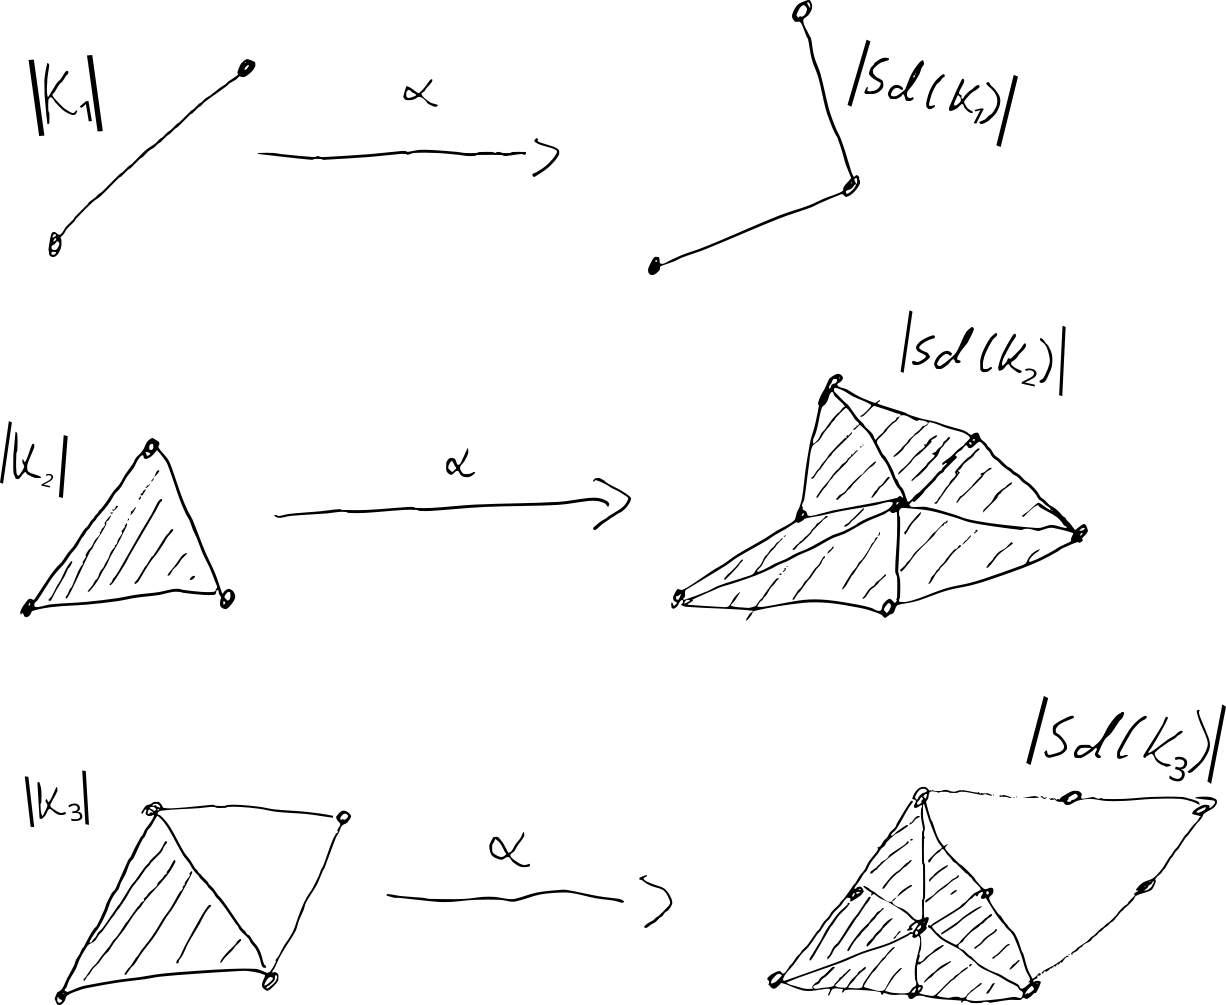
\includegraphics[width=0.8\textwidth]{png/Alpha.png}
		\end{center}
		\caption{Tre døme av barysentriske oppdelingar.}
		\label{fig:alpha}
	\end{figure}
\end{example}

\begin{lemma} \label{thm:konveks-kombinasjon-i-konveks}
	La \( V \) vera ei konveks mengd, og la \( P := \set{p_1, p_2, \dots, p_n } \) vera (ikkje nødvendegvis geometrisk uavhengige) punkt i \( V \).
	
	Då er alle konvekse kombinasjonar av \( P \) inneheldt i \( V \).
\end{lemma}

\begin{proof}
	Beviset er gjort ved induksjon på talet på punkt i mengda av punkt ein tek ein koveks kombinasjon over, her kalla \( n \).

	Ein vis fyrst grunntilfella:

	La \( n = 1 \), då er \( x = a_1 p_1 \), med \( a_1 = 1 \), så \( x = p_1 \in K \).
	
	For \( n = 2 \), då er \( x = a_1 p_1 + a_2 p_2 \), med \( a_1 + a_2 = 1 \). Men då er \( a_2 = 1 - a_1 \), så ein kan skriva \( x = a_1 p_1 + (1-a_1) p_2 \). Men dette er jo definisjonen på eit punkt på eit linjestykke mellom \( p_1 \) og \( p_2 \). Så frå definisjonen av ei konveks mengd, så må \( x \in K \).

	Anta det gjeld for \( n = k-1 \), ein vil no visa at det gjeld for \( n = k \).

	La \( x = \sum_{i=1}^k a_i p_i \). Ein kan då skriva
	\[ 
		x = a_1 p_1 + \sum_{i=2}^k a_i p_i = a_1 p_1 + (\sum_{i=2}^k a_i) \frac{\sum_{i=2}^k a_i p_i}{(\sum_{i=2}^k a_i)} = a_1 p_1 + (1-a_1) \frac{\sum_{i=2}^k a_i p_i}{(\sum_{i=2}^k a_i)}.
	\]
	Ein ser at
	\[
		\frac{\sum_{i=2}^k a_i p_i}{(\sum_{i=2}^k a_i)} = \sum_{i=2}^k p_i\frac{a_i}{(\sum_{i=2}^k a_i)}
	\]
	dannar ein konveks kombinasjon av \( k-1 \) punkt sidan
	\[
		\sum_{i=2}^k \frac{a_i}{(\sum_{i=2}^k a_i)} = \frac{\sum_{i=2}^k a_i}{(\sum_{i=2}^k a_i)} = 1
	\]
	og
	\[
		\frac{a_i}{(\sum_{i=2}^k a_i)} \geq 0, \, i=2,3,\dots,k.
	\]
	Difor er
	\[
		y := \frac{\sum_{i=2}^k a_i p_i}{(\sum_{i=2}^k a_i)}
	\]
	eit element i \( V \) av induksjonshypotesen. Og ein har at
	\[
		x = a_1 p_1 + \sum_{i=2}^k a_i p_i = a_1 p_1 + (1-a_1) y
	\]
	er ein konveks kombinasjon av \( 2 \) punkt i \( V \), og ein får frå induksjonshypotesen at \( x \in V \).
\end{proof}

\begin{definition} \label{thm:Gamma}
	La \( U = \set{U_i}_{i=1}^n \) vera ei endeleg mengd av konvekse delmengder av \( \Rb^m \). Vidare, for kvar \( \epsilon \in \Nc(U) \) vel eit punkt \( v_\epsilon \in \intersect_{u \in \epsilon} u \). Vidare, la \( x \in \gr{\Sd(\Nc(U))}_f \) vera ein konveks kombinasjon av dei geometrisk uavhengige punkta \( f(\sigma) \) for ein eller annan \( \sigma \in \Sd(\Nc(U)) \), der \( \sigma = \tuple{\sigma_1, \sigma_2, \dots, \sigma_{\#\sigma}} \) med dei barysentriske koordinatane \( \tuple{a_1, a_2, \dots, a_{\#\sigma}} \).
	
	Definér då
	\begin{align*}
		\Gamma : \gr{\Sd(\Nc(U))}_f &\to \union_{u \in U} u \\
		x &\mapsto \sum_{i=1}^{\#\sigma} a_i v_{\sigma_i}.
	\end{align*}
\end{definition}

\begin{lemma} \label{thm:Gamma-eigenskapar}
	Avbildinga \( \Gamma \) frå \autoref{thm:Gamma} er veldefinert, kontinuerleg og biletet er i \( \union_{u\in U} u \).
\end{lemma}

\begin{proof}
	Avbildinga \( \Gamma \) er kontinuerleg og veldefinert på ulike representasjonar av verdiar, fordi om ein lar \( \hat{\tau} : \gr{\Sd(\Nc(U))}_f \to \gr{\Sd(\Nc(U))}_{\hat{\tau} \circ f} \) vera definert som i \autoref{thm:tau-homeomorfi} (\( x \mapsto x - f(\hat{\sigma}) \) for ein \( \hat{\sigma} \in \Nc(U) \)), så er dette ein homeomorfi, og om ein deretter definerer \( L \) til å vera ein lineæravblildning som tek \( \hat{\tau} \circ f (\sigma) \mapsto v_{\sigma} \) for alle \( \sigma \in \Nc(U) \). Og vidare la \( \hat{L} := L|_{\gr{\Sd(\Nc(U))}_{\hat{\tau}\circ f}} \), så ser ein at for \( x \in \gr{\Sd(\Nc(U))}_f \) ein konveks kombinasjon av dei geometrisk uavhengige punkta \( f(\sigma) \) for ein eller annan \( \sigma \in \Sd(\Nc(U)) \), der \( \sigma = \tuple{\sigma_1, \sigma_2, \dots, \sigma_{\#\sigma}} \) med dei barysentriske koordinatane \( \tuple{a_1, a_2, \dots, a_{\#\sigma}} \) så er
	\begin{align*}
		\hat{L} \circ \hat{\tau} (x) &= \hat{L} \circ \hat{\tau} \tuple{\sum_{i=1}^{\#\sigma}a_i f(\sigma_i)} \\
		&= \hat{L} \tuple{\sum_{i=1}^{\#\sigma}a_i f(\sigma_i)-f(\hat{\sigma})} \\
		&= \hat{L} \tuple{\sum_{i=1}^{\#\sigma}a_i f(\sigma_i)-\tuple{\sum_{j=1}^{\#\sigma}a_i}f(\hat{\sigma})} \\
		&= \hat{L} \tuple{\sum_{i=1}^{\#\sigma}a_i f(\sigma_i)-\tuple{\sum_{j=1}^{\#\sigma}a_if(\hat{\sigma})}} \\
		&= \hat{L} \tuple{\sum_{i=1}^{\#\sigma}a_i\tuple{f(\sigma_i)-f(\hat{\sigma})}} \\
		&= \hat{L} \tuple{\sum_{i=1}^{\#\sigma}a_i\hat{\tau}\tuple{f(\sigma_i)}} \\
		&= \sum_{i=1}^{\#\sigma}a_iL\tuple{\hat{\tau}\tuple{f(\sigma_i)}} \\
		&= \sum_{i=1}^{\#\sigma}a_i v_{\sigma_i} \\
		&= \Gamma(x)
	\end{align*}
	og sidan \( \hat{\tau} \) er kontinuerleg og veldefinert, og \( \hat{L} \) er kontinuerleg og veldefinert frå \autoref{thm:avgrensa-lin-op-er-kont} og \autoref{thm:universal-eigenskap-underromstopologi}, så må \( \Gamma = \hat{L}\circ\hat{\tau} \) også vera kontinuerleg og veldefinert.

	Biletet til \( \Gamma \) er i \( \union_{u\in U} u \), fordi for \( x \in \gr{\Sd(\Nc(U))}_f \) ein konveks kombinasjon av dei geometrisk uavhengige punkta \( f(\sigma) \) for ein eller annan \( \sigma \in \Sd(\Nc(U)) \), der \( \sigma = \tuple{\sigma_1, \sigma_2, \dots, \sigma_{\#\sigma}} \) med dei barysentriske koordinatane \( \tuple{a_1, a_2, \dots, a_{\#\sigma}} \), så får ein at
	\[
		\Gamma(x) = \sum_{i=1}^{\#\sigma} a_i v_{\sigma_i}
	\]
	er ein konveks kombinasjon av punkta \( v_{\sigma_i} \) for \( i = 1,2,\dots,\#\sigma \). Men sidan \( \sigma_1 \subsetneq \sigma_2 \subsetneq \dots \subsetneq \sigma_{\#\sigma} \), så er det ein \( \epsilon \in U \) med \( \epsilon \in \sigma_1, \sigma_2, \dots, \sigma_{\#\sigma} \). Og difor er \( v_{\sigma_1}, v_{\sigma_2}, \dots, v_{\sigma_{\#\sigma}} \in \epsilon \). Men ettersom alle elementa i \( U \) er konvekse mengder, så er \( \Gamma(x) \) ein konveks kombinasjon av element i ei konveks mengd, \( \epsilon \), og frå \autoref{thm:konveks-kombinasjon-i-konveks}, så er \( x \in \epsilon \subseteq \union_{u\in U} u \).
\end{proof}

\begin{example}
	I \autoref{fig:Gamma} så kan ein sjå korleis \( \Gamma \) avbildinga fungerar på den barysentriske oppdelinga av ei samling av konvekse mengder. Merk her desse farga områda, dei blir viktige i framtida.
	\begin{figure}[htbp]
		\begin{center}
			\includesvg[width=0.8\textwidth]{Gamma.svg}
		\end{center}
		\caption{Avbildinga \( \Gamma \).}
		\label{fig:Gamma}
	\end{figure}
\end{example}

\begin{definition}
	La \(  U=\set{U_i}_{i=1}^n \) vera ei mengd av delmengder av \( \Rb^d \), og la \( \epsilon > 0 \).
	
	Definér \( U_i^\epsilon := \union_{x \in U_i} B_\epsilon(x) \), og definér \( U^\epsilon := \set{U_i^\epsilon}_{i=1}^n \).
\end{definition}

\begin{lemma} \label{thm:epsilondekke}
	La \( U = \set{U_i}_{i=1}^n \) vera ei endeleg mengd av kompakte delmengder av \( \Rb^d \), og la \( A \) vera mengda av alle mogelge delmengder av \( U \), og la \( A^\epsilon \) vera mengda av alle mogelge delmengder av \( U^\epsilon \). La
	\begin{align*}
		f: A &\to A^\epsilon \\
		\set{U_{i_1}, U_{i_2}, \dots, U_{i_k}} &\mapsto \set{U_{i_1}^\epsilon, U_{i_2}^\epsilon, \dots, U_{i_k}^\epsilon}.
	\end{align*}
	
	Då eksisterer det ein \( \epsilon > 0 \) sånn at
	\[
		f|_{\Nc(U)}: \Nc(U) \to \Nc(U^\epsilon)
	\]
	er ein bijeksjon.
\end{lemma}

\begin{proof}
	 Ein ser at \( f \) dannar ein bijeksjon frå \( A \) til \( A^\epsilon \). Og sidan \( i: \Nc(U) \hookrightarrow A \), inklusjonsavbildinga, er injektiv, så er \( f \circ i \) injektiv.

	Ettersom \( U^{\epsilon} \) kan berre få fleire snitt, enn \( U \), så må \( f(\Nc(U)) \subseteq \Nc(U^{\epsilon}) \).
	
	For å visa \( f(\Nc(U)) \supseteq \Nc(U^{\epsilon}) \), så ser ein på det kontrapostive tilfellet:
	 
	\begin{align*}
		f(\Nc(U)) &\supseteq \Nc(U^{\epsilon}) \\
		&\Updownarrow \\ 
		\forall \sigma \in \Nc(U^{\epsilon}) &\implies \sigma \in f(\Nc(U)) \\
		&\Updownarrow \\
		\forall \sigma \in A, \sigma \not\in f(\Nc(U)) &\implies \sigma \in A^\epsilon, \sigma \not\in \Nc(U^{\epsilon})
	\end{align*}

	For ein \( \sigma = \set{U_{i_1}, U_{i_2}, \dots, U_{i_k}} \in A \) så kan ein skriva det som \( \sigma_J \) for \( J = \set{i_1, i_2, \dots i_k} \). Likt for \( \sigma^\epsilon_J \in A^\epsilon \). Så ein vil visa at \( \exists \epsilon : \sigma^\epsilon_J \not\in f(\Nc(U)) \implies \sigma^\epsilon_J \not\in \Nc(U^{\epsilon}) \) for alle moglege \( J \) der \( \sigma^\epsilon_J \not\in f(\Nc(U)) \). Men ettersom \( f \) dannar ein bijeksjon frå \( A \) til \( A^\epsilon \), så kan ein sjå på \( \exists \epsilon : \sigma_J \not\in \Nc(U) \implies f(\sigma_J) \not\in \Nc(U^{\epsilon}) \).

	La
	\[
		r_J := \sup_{x \in \union_{j \in J} u_j} d(x,0).
	\]
	Sidan \( \union_{j \in J} u_j \) er ein endeleg union av kompakte mengder så er den kompakt frå \autoref{thm:endeleg-union-kompakt-er-kompakt}. Då får ein frå \autoref{thm:supremum-over-kompakt-er-maks}, at \( r_J = \max_{x \in \union_{j \in J} u_j} d(x,0) \) og difor endeleg. Ein får også at \( \union_{j \in J} u_j \subseteq \bar{B}_{r_J}(0) \).
	
	Definer vidare \( D_J := \bar{B}_{4r_J}(0) \). Sidan dette er ein lukka og avgrensa mengd i \( \Rb^d \), så er den kompakt frå \autoref{thm:heine-borel}.

	La \( g_J: D_J \to \Rb \) der \( x \mapsto \max_{j \in J} d(x, U_j) \). 
	
	La \( Z_k := \set{x \in D_J: d(x, U_k) = g_J(x)} \), då er den lukka fordi for \( x_n \in Z_k \) der \( \set{x_n}_{n\in\Nb} \to x \), så har ein at \( \set{d(x_n, U_k)}_{n\in\Nb} \to d(x, U_k) \) fordi \( d(x, U_k) \) er kontinueleg frå \autoref{thm:distanse-er-kont}. Så annta at følga konvergerte utanfor \( Z_k \), altså \( g_J(x) > d(x, U_k) \). Då er \( g_J(x)-d(x, U_k) = \epsilon > 0 \). Men då er \( |d(x, U_k)-d(x_n, U_k)| \geq \epsilon \) sidan \( d(x_n, U_k) \geq g_J(x) > d(x, U_k) \). Men dette strider imot at \( \set{d(x_n, U_k)}_{n\in\Nb} \to d(x, U_k) \), så \( Z_k \) må vera lukka.
	
	Då ser ein at \( g_J \) er kontinuerleg, fordi om ein ser på \( g_J|_{Z_k} \), så er jo dette kun \( d(x, U_k) \), som er kontinuerleg frå \autoref{thm:distanse-er-kont}, om ein gjentek dette for alle \( Z_k \) for \( k \in J \), så gir \autoref{thm:pasting-lemma} at \( g_J \) er kontinuerleg.

	Om ein lar \( \sigma_J \not\in \Nc(U) \), så får ein at \( g_J(x) > 0 \) for alle \( x \) i \( D_J \), sidan \( \intersect_{u \in \sigma_J} u = \emptyset \).

	Og sidan \( D_J \) er kompakt, så får ein frå \autoref{thm:infimum-over-kompakt-er-min}, at \( g_J(x) \) oppnår eit minimum, som frå argumentet ovanfor må vera ulik \( 0 \). Dette kallar ein for
	\[
		\epsilon_J := \min_{x \in D_J} \max_{j \in J} d(x, U_j).
	\]
	Men dette minimumet er eit globalt minimum over heile \( \Rb^d \), fordi for \( x \in \Rb^d \setminus D_J \), så er \( g_J(x) \geq 3r_J \), sidan det er minste moglege avstand frå \( x \) til ei av \( u_j \in U_J \). Men om \( x \in \bar{B}_{r_J}(0) \) då er \( g_J(x) \leq 2r_J \) sidan det er det lengste vekke den andre mengda kan vera og framleis vera inne i \( \bar{B}_{r_J}(0) \). Så eit globalt minimum må vera eit minimum inne i \( D_J \).

	Vidare så ser ein at \( \sigma_J^{\epsilon_J} \not\in \Nc(U^{\epsilon_J}) \) fordi om ein lar \( x \) vera eit av punkta som gav det globale minimumet \( \epsilon_J \), så er \( x \not\in \intersect_{j \in J} u_j^{\epsilon_J} \) fordi det er ingen \( y \in  u_{\hat{j}} \) for \( \hat{j} \) den verdien i \( J \) som gav maksimumet til \( \max_{j \in J} d(x, U_j) \), som har \( d(y, x) > \epsilon_J \). Så det er ingen open ball om \( y \) med radius \( r_J \) som inneheld \( x \). Difor kan ikkje \( x \) vera i snittet av alle \( u_j \)-ane. Det same argumentet gjeld for alle andre punkt i \( D_J \) som ikkje var globale minimum.
	
	Så det er ingen punkt i \( \intersect_{j \in J} u_j^{\epsilon_J} \), og difor er \( \sigma_J^{\epsilon_J} \not\in \Nc(U^{\epsilon_J}) \).

	Vidare, la
	\[
		\epsilon := \min_{\set{J : \sigma_J \not\in \Nc(U)}} \epsilon_J.
	\]
	Då er \( \epsilon \neq 0 \) fordi alle \( \epsilon_J \neq 0 \) og det er berre endeleg mange \( \sigma_J \in A \).

	Om ein brukar den øvre \( \epsilon \)-en så får ein at for alle \( \sigma_J \not\in \Nc(U) \), så er \( \sigma_J^{\epsilon}=f(\sigma_J) \not\in \Nc(U^{\epsilon}) \), som var det ein ville visa.
\end{proof}

\begin{remark}
	Avbildinga \( f \) ovanfor, blir ofte kalla ein simplisiell isomorfi, og er det eg peika til når eg skreiv at nerva til \( \set{\set{\bar{B}_\epsilon(p_i)}}_{i=1}^n \) var ekvivalent med Cech-komplekset av \( \set{p_i}_{i=1}^n \) med radius \( \epsilon \) i \autoref{rem:cech-ekvivalent}.
\end{remark}

\begin{definition} \label{def:psi}
	La \( U = \set{U_i}_{i=1}^n \) vera ei endeleg mengd av kompakte delmengder av \( \Rb^d \), og la \( \epsilon \) vera som i \autoref{thm:epsilondekke}.

	Definér då
	\begin{align*}
		\phi_i : \union_{u \in U} u &\to [0, \infty) \\
		x &\mapsto \frac{d(x, \Rb^m \setminus U_i^\epsilon)}{d(x, U_i) + d(x, \Rb^m \setminus U_i^\epsilon)}
	\end{align*}
	og vidare
	\begin{align*}
		\psi_i : \union_{u \in U} u &\to [0, 1] \\
		x &\mapsto \frac{\phi_i(x)}{\sum_{k=1}^n \phi_k(x)}.
	\end{align*}
\end{definition}

\begin{lemma}
	Avbildingene \( \phi_i \) og \( \psi_i \) frå \autoref{def:psi} er kontinuerlege og veldefinerte.
\end{lemma}

\begin{proof} 
	Sidan avstandsfunksjonen \( d \) er kontinuerleg frå \autoref{thm:distanse-er-kont}, og nemnaren er alltid ulik null sidan \( U_i \subsetneq U_i^\epsilon \) og ein sum av to kontinuerlege funskjonar og difor kontinuerleg sjølv, så er \( \phi_i \) ein kvotient av to kontinuerlege funskjonar med heile \( \Rb^d \) som definisjonsmengd, og difor kontinerleg på \( \union_{i=1}^n U_i \) frå \autoref{thm:universal-eigenskap-underromstopologi}.

	Ved mykje det same argumentet så ser ein at \( \psi_i \) er ein kvotient med ein kontinuerleg avbilding i teljaren og ein sum av kontinerlege avbildinger som er alltid ulik null på \( \union_{i=1}^n U_i^\epsilon \) sidan minst ein \( \phi_i \) er ulik null fordi \( \phi_i(x)=0 \) berre når \( d(x, \Rb^m \setminus U_i^\epsilon)=0 \) som skjer når \( x \not\in U_i^\epsilon \). Men sidan for \( x \in \union_{i=1}^n U_i \) så er det vertfall ein \( U_i^\epsilon \) som \( x \) er eit element av. Difor er \( \psi_i \) kontinerleg.

	I tillegg, for \( \phi_i(x) \neq 0 \), så er
	\[
		\psi_i(x) = \frac{\phi_i(x)}{\sum_{k=1}^n \phi_k(x)} \leq \frac{\phi_i(x)}{\phi_i(x)} = 1,
	\]
	så verdimengda til \( \psi_i \) er veldefinert.
\end{proof}

\begin{definition} \label{def:Psi}
	La \( U = \set{U_i}_{i=1}^n \) vera ei endeleg mengd av kompakte delmengder av \( \Rb^d \), og la \( \psi_i \) vera som i \autoref{def:psi}, og \( f: U \to \Rb^d \) ei affin imbedding. 
	
	Definer for \( x \in \union_{u \in U} u \):
	\begin{align*}
		\Psi : \union_{u \in U} u &\to \gr{\Nc(U)} \\
		x &\mapsto \sum_{i=1}^n \psi_i(x)f(U_i)
	\end{align*}
\end{definition}

\begin{lemma} \label{thm:psi-kont}
	Avbildinga \( \Psi \) frå \autoref{def:Psi} er kontinuerleg, og har bilete i \( \gr{\Nc(U)}_f \).
\end{lemma}

\begin{proof}
	Sidan alle \( \psi_i \)-ane er kontinuerlege, så er \( \psi_i(x) f(U_i) \) også kontinuerleg, ettersom \( f(U_i) \) er ein konstant vektor. Så \( \Psi \) er ein sum av kontinuerlege funksjonar og difor kontinuerleg sjølv.

	For å visa at \( \Psi\tuple{\union_{u \in U} u} \subseteq \gr{\Nc(U)}_f \), la \( x \in \union_{u \in U} u \). Då er \( \Psi(x) = \sum_{i=1}^n \psi_i(x)f(U_i) \). Merk at:
	\begin{align*}
		\sum_{j=1}^n \psi_j(x)  &= \sum_{j=1}^n \frac{\phi_j(x)}{\sum_{k=1}^n \phi_k(x)} \\
		&= \frac{\sum_{j=1}^n \phi_j(x)}{\sum_{k=1}^n \phi_k(x)} \\
		&= 1.
	\end{align*}
	Sidan \( \phi_i(x) \geq 0 \) for alle \( i \) og \( x \) så er \( \psi_i(x) \geq 0 \) for alle \( i \) og \( x \). Difor så får ein at \( \Psi(x) \) er ein konveks kombinasjon av punkta \( f(U) \).

	Ettersom \( x \not\in U_i^\epsilon \iff \phi_i(x) = 0 \iff \psi_i(x) = 0 \), så får ein at \( \psi_i(x) \neq 0 \iff x \in U_i^\epsilon \). La då \( A_x^\epsilon := \set{U_i^\epsilon \in U^\epsilon : x \in U_i^\epsilon} \). Då ser ein at \( A_x^\epsilon \in \Nc(U^\epsilon) \). Men med \( h(x) \) bijeksjonen ein får frå \autoref{thm:epsilondekke}, så veit ein at \( A_x^\epsilon \) korrsponderar til ein \( A_x := h^{-1}(A_x^\epsilon) \in \Nc(U) \).
	
	Så for alle \( x \in \union_{u \in U} u \) så er \( \Psi(x) \) ein konveks kombinasjon av punkta \( f(A_x) \), altså \( x \in \gr{A_x}_f \subseteq \gr{\Nc(U)}_f \), sidan \( A_x \in \Nc(U) \). Difor er biletet til \( \Psi \) i \( \gr{\Nc(U)}_f \).
\end{proof}

\begin{definition} \label{def:bst}
	La \( K \) vera eit endeleg abstrakt simplisielt kompleks over \( V \), og la \( v \) vera eit vilkårleg element i \( V \).
	
	Då er \emph{den lukka barysentriske stjerna til \( K \) i \( v \)}, skrive \( \bst(v) \), gitt ved
	\[
		\bst(v) = \set{\sigma \in \Sd(K) \mid \sigma \union \set{v} \in \Sd(K)}.
	\]
\end{definition}

\begin{example}
	Den barysentriske stjerna er nøyaktig dei farga delane ein såg i \autoref{fig:Gamma} over. Merk her at \( \Gamma \) ser ut til å alltid ta ein barysentrisk stjerne fullstendig inni eine mengda i biletet. Det blir viktig i beviset av Nerveteoremet.
\end{example}

\begin{lemma} \label{thm:bst-ask}
	Den lukka barysentriske stjerna som definert i \autoref{def:bst}, er eit abstrakt simplisielt kompleks med hjørnemengd \( W = \set{w \in K : \set{w} \union \set{v} \in \Sd(K)} \).
\end{lemma}

\begin{proof}
	Her må ein visa dei tre eigenskapane frå \autoref{def:ASK} held:
	\begin{enumerate}
		\item{For \( w \in W \), så er \( \set{w} \in \bst(v) \) frå definisjonen.}
  		\item{For \( \sigma \in \bst(v) \) så er \( \sigma \subseteq W \), fordi for ein vilkårleg \( \tau \in \sigma \), så er \( \sigma \union \set{v} = \set{\tau} \union \sigma \union \set{v} \in \Sd(K) \). Men sidan \( \Sd(K) \) er eit abstrakt simplisielt kompleks frå \autoref{thm:subdivisjon-abstrakt-simplisielt-kompleks}, så er \( \sigma \union \set{v} \supseteq \set{\tau} \union \set{v} \in \Sd(K) \). Og då er \( \tau \in W \).}
    	\item{For \( \sigma \in \bst(v) \), la \( \tau \subseteq \sigma \). Sidan \( \sigma \union \set{v} \in \Sd(K) \), og sidan \( \Sd(K) \) er eit abstrakt simplisielt kompleks frå \autoref{thm:subdivisjon-abstrakt-simplisielt-kompleks}, så er \( \sigma \union \set{v} \supseteq \tau \union \set{v} \in \Sd(K) \). Difor er \( \tau \in \bst(v) \).}
	\end{enumerate}
\end{proof}

\begin{lemma} \label{thm:Gamma-inni-ui}
	La \( U = \set{U_i}_{i=1}^n \) vera ei endeleg mengd av konvekse mengder i \( \Rb^m \), og la \( \Gamma \) vera definert som i \autoref{thm:Gamma}.

	Då er \( \Gamma(\gr{\bst(U_i)}_f) \subseteq U_i \).
\end{lemma}

\begin{proof}
	Frå \autoref{thm:bst-ask}, så veit ein at hjørnemengda til \( \bst(U_i) \), er
	\[
		W = \set{w \in \Nc(U) : \set{w} \union \set{U_i} \in \Sd(\Nc(U))}=\set{w \in \Nc(U) : U_i \in w}.
	\] 
	Men då er jo \( v_w \) (frå \autoref{thm:Gamma}) eit element i \( \intersect_{u \in w} u \subseteq U_i \) for alle \( w \). Og sidan \( \Gamma \) tek eit element, \( x \), i \( \gr{\bst(U_i)}_f \) som er ein konveks kombinasjon av punkta \( \set{f(w)}_{w \in W} \) til ein konveks kombinasjon av \( \set{v_w}_{w \in W} \subseteq U_i \), så får ein at \( \Gamma(x) \) er ein konveks kombinasjon av punkta \( \set{v_w}_{w \in W} \), som alle ligg i ei konveks mengd \( U_i \), og ein får difor frå \autoref{thm:konveks-kombinasjon-i-konveks} at \( x \in U_i \).
\end{proof}

\begin{lemma} \label{thm:bst-betingingar}
	La \( U = \tuple{U_i}_{i=1}^n \) vera ei endeleg mengd av delmengder av \( \Rb^d \), og la \( \alpha: \gr{\Sd(\Nc(U))}_f \to \gr{\Nc(U)}_g \) vera definert som i \autoref{thm:alpha-homeomorfi}. Vidare, la \( x \in \gr{\Nc(U)}_g \) vera ein konveks kombinasjon av punkta \( g(\tau) \) for ein eller annan \( \tau \in \Nc(U) \) med barysentriske koordinatar \( \tuple{b_1, b_2,\dots, b_i, \dots, b_{\#\tau}} \). La \( b_i \geq b_j, \, \forall j \in \set{1, 2, 3, \dots, \#\tau} \). 
	
	Då er
	\[ 
		\alpha^{-1}(x) \in \gr{\bst(U_i)}.
	\]
\end{lemma}

\begin{proof}
	Fyrst merk at
	\[
		\alpha^{-1} = \tau_f^{-1} \circ \tilde{L} \circ \tau_g
	\]
	så ein får at
	\begin{align*}
		\alpha^{-1}(x) &= \tau_f^{-1} \circ \tilde{L} \circ \tau_g (x) \\
		&= \tau_f^{-1} \circ \tilde{L} \circ \tau_g \tuple{\sum_{j=1}^{\#\tau} b_j g(U_j)}. \\
		\intertext{Sidan \( \tau_g \) bevarer barysentriske koordinatar frå beviset til \autoref{thm:tau-homeomorfi} har ein at}
		\tau_f^{-1} \circ \tilde{L} \circ \tau_g \tuple{\sum_{j=1}^{\#\tau} b_j g(U_j)} &= \tau_f^{-1} \circ \tilde{L} \tuple{\sum_{j=1}^{\#\tau} b_j \tau_g \circ g(U_j)}.
	\end{align*}
	Men frå antakinga så har ein at \( b_i \geq b_j \, \forall j \in \set{1, 2, 3, \dots, \#\tau} \). Så ein kan vela ei ordning av \( U = \tuple{U_{j_i}}_{i=1}^n \) sånn at \( b_{j_1} \geq b_{j_2} \geq b_{j_3} \geq \dots \geq b_{j_{\#\tau}} \), og der \( b_{j_1}=b_i \). Ein har då 
	\[
		\sigma = \tuple{\sigma_i}_{i=1}^{\#\tau} = \tuple{\union_{i=1}^k \set{U_{j_i}}}_{k=1}^{\#\tau}.
	\]
	La \( a_k = k\tuple{b_{j_k}-b_{j_{k+1}}} \), då får ein at
	\begin{align*}
		\alpha^{-1}(x) &= \tau_f^{-1} \tuple{\sum_{l=1}^{\#\tau}a_k \tau_f \circ f(\sigma_i)} \\
		&= \sum_{l=1}^{\#\tau} a_k f(\sigma_i).
	\end{align*}
	Men sidan \( \sigma \in \bst(U_i) \) sidan \( \sigma \union \set{U_i} = \sigma \in \Sd(\Nc(U)) \), og \( \sum_{k=1}^{\#\tau} a_k = 1 \), og \( a_k \geq 0, \, \forall k \) frå beviset til \autoref{thm:alpha-homeomorfi}. Så er \( \alpha(x) \) ein konveks kombinasjon av punkta i \( f(\sigma), \sigma \in \bst(U_i) \), og difor er
	\[
		\alpha^{-1}(x) \in \gr{\bst{U_i}}_f. \qedhere
	\]
\end{proof}

\begin{lemma} \label{thm:Psi-inni-bst}
	La \( U = \set{U_i}_{i=1}^n \) vera ei endeleg mengd av kompakte delmengder av \( \Rb^m \) og la \( \Psi \) vera som i \autoref{def:Psi}. Vidare, la \( f: \Nc(U) \to \Rb^d \) vera ei affin imbedding, og la \( \alpha \) vera som i \autoref{thm:alpha-homeomorfi}.

	Då er \( \alpha \circ \Psi(U_i) \subseteq \gr{\bst(U_i)}_f \).
\end{lemma}

\begin{proof}
	La \( x \in U_i \). Då ser ein at
	\[
		\phi_i(x) = \frac{d(x, \Rb^m \setminus U_i^\epsilon)}{d(x, U_i) + d(x, \Rb^m \setminus U_i^\epsilon)} = \frac{d(x, \Rb^m \setminus U_i^\epsilon)}{d(x, \Rb^m \setminus U_i^\epsilon)} = 1.
	\] 
	For \( j \neq i \), sidan \( d(x, U_j) \geq 0 \), så får ein
	\[
		\phi_j(x) = \frac{d(x, \Rb^m \setminus U_j^\epsilon)}{d(x, U_j) + d(x, \Rb^m \setminus U_j^\epsilon)} \leq \frac{d(x, \Rb^m \setminus U_j^\epsilon)}{d(x, \Rb^m \setminus U_j^\epsilon)} = 1
	\]
	så \( \phi_i(x) \geq \phi_j(x) \) for alle \( j \).

	Dette gir at
	\[
		\psi_i(x) = \frac{\phi_i(x)}{\sum_{k=1}^n \phi_k(x)} \geq \frac{\phi_j(x)}{\sum_{k=1}^n \phi_k(x)} = \psi_j(x).
	\]
	La \( \tau = \set{U_i : \psi_i(x) \neq 0} \in \Nc(U) \).

	Sidan \( \Psi(x) \) er ein konveks kombinasjon av punkta \( f(\tau) \) med barysentriske koordinatar \( A:= \tuple{\psi_j(x)}_{\set{ j : U_j\in \tau}} \) (frå beviset til \autoref{thm:psi-kont}), og sidan \( \psi_i(x) \neq 0 \), så er \( U_i \in \tau \), og \( \psi_i(x) \in A \).
	
	Frå det som vart vist ovanfor, så er \( \phi_i(x) \geq \phi_j(x) \) for alle \( \phi_j(x) \in A \).
	
	Så frå \autoref{thm:bst-betingingar}, så er
	\[
		\alpha \circ \Psi(x) \in \gr{\bst(U_i)}_f.
	\]
	Sidan dette var uavhengig av val av \( x \in U_i \) så får ein
	\[
		\alpha \circ \Psi(U_i) \subseteq \gr{\bst(U_i)}_f. \qedhere
	\]
\end{proof}

\begin{lemma} \label{thm:homeq-u}
	La \( U = \tuple{U_i}_{i=1}^n \) vera ei endeleg mengd av kompakte og konvekse delmengder av \( \Rb^d \). La \( \Gamma \) vera som i \autoref{thm:Gamma}, la \( \Psi \) vera som i \autoref{def:Psi}, og la \( \alpha \) vera som i \autoref{thm:alpha-homeomorfi}. 
	
	Då er
	\[
		\Gamma \circ \alpha^{-1} \circ \Psi \simeq \Id_{\union_{u \in U} u}.
	\]
\end{lemma}

\begin{proof}
	For \( x \in U_i \) så følger det frå \autoref{thm:Psi-inni-bst} at
	\[
		\alpha^{-1} \circ \Psi(x) \in \gr{\bst(U_i)}_f.
	\]
	Frå \autoref{thm:Gamma-inni-ui} så får ein difor at
	\[
		\Gamma \circ \alpha^{-1} \circ \Psi(x) \in U_i.
	\]
	Sjå på avbildinga
	\begin{align*}
		H: \union_{u \in U} u \times I &\to \union_{u \in U} u \\
		\tuple{x, t} &\mapsto xt + \Gamma \circ \alpha^{-1} \circ \Psi(x)(1-t)
	\end{align*}
	Denne er kontinuerleg fordi \( \Gamma \) er kontinuerleg frå \autoref{thm:Gamma-eigenskapar}, \( \Psi \) er kontinuerleg frå \autoref{thm:psi-kont}, og \( \alpha \) er ein homeomorfi.
	
	Den er også veldefinert fordi om ein fikserar ein \( x \in U_i \) så er \( xt + \Gamma \circ \alpha^{-1} \circ \Psi(x)(1-t) \in U_i \) for alle \( t \in I \) sidan det er på ei linje mellom to punkt i \( U_i \) som er konveks.

	Så \( H \) er ein homotopi frå \( \Id_{\union_{u \in U} u} \) til \( \Gamma \circ \alpha^{-1} \circ \Psi \).
\end{proof}

\begin{definition}
	La \( K \) vera eit endeleg abstrakt simplisielt kompleks over hjørnemengda \( V \). 
	
	Då er \emph{\( n \)-skjelettet} til \( K \), skrive \( \Sk_n(K) \), gitt ved
	\[
		\Sk_n(K) := \set{\sigma \in K : \#\sigma \leq n}.
	\]
\end{definition}

\begin{lemma}
	La \( K \) vera eit endeleg abstrakt simplisielt kompleks over hjørnemengda \( V \). 
	
	Då er \( n \)-skjelettet til \( K \) eit abstrakt simplisielt kompleks.
\end{lemma}

\begin{proof}
	Alle \( \tau \in \Sk_n(K) \) er delmengder av ein \( \sigma \in K \), så dei oppfyllar krav 2 og 3 av \autoref{def:ASK}. Krav 1 er oppfylt ved at \( \Sk_0(K) \subseteq \Sk_n(K) \).
\end{proof}

\begin{lemma} \label{thm:konveks-kombinasjon-er-konveks}
	La \( V := \set{v_1, v_2, \dots, v_n} \subseteq \Rb^d \) vera ei mengda av punkt.
	
	Då er det geomeriske simplekset utspent av \( V \) konveks.
\end{lemma}

\begin{proof}
	La \( \Delta \) vera det geometriske simplekset. La \( x \) og  \( y \) vera to vilkårlege punkt i \( \Delta \). Då er
	\[
		x = \sum_{i=1}^n a_i v_i
	\]
	og
	\[
		y = \sum_{i=1}^n b_i v_i
	\]
	med \( a_i, b_i \geq 0 \, \forall i \), og difor er
	\[
		\sum_{i=1}^n a_i = \sum_{i=1}^n b_i = 1.
	\]
	For ein vilkårleg \( t \in I \), sjå på
	\begin{align*}
		xt + (1-t)y &= t \sum_{i=1}^n a_i v_i + (1-t)\sum_{i=1}^n b_i v_i \\
		&= \sum_{i=1}^n b_i v_i +t\tuple{\sum_{i=1}^n a_i v_i-\sum_{i=1}^n b_i v_i} \\
		&= \sum_{i=1}^n b_i v_i +t\tuple{\sum_{i=1}^n (a_i-b_i) v_i} \\
		&= \sum_{i=1}^n b_i v_i +\tuple{\sum_{i=1}^n t(a_i-b_i) v_i} \\
		&= \sum_{i=1}^n b_i v_i +t(a_i-b_i) v_i \\
		&= \sum_{i=1}^n (b_i+t(a_i-b_i)) v_i.
	\end{align*}
	Merk fyrst at \( b_i+t(a_i-b_i) \geq 0 \) fordi 
	\[ 
		b_i+t(a_i-b_i) = (1-t)b_i+ta_i \geq ta_i \geq 0.
	\]
	Vidare så er
	\begin{align*}
		\sum_{i=1}^n (b_i+t(a_i-b_i)) &= \sum_{i=1}^n (1-t)b_i+ta_i \\
		&= (1-t)\sum_{i=1}^n b_i + t \sum_{i=1}^n a_i \\
		&= 1 - t + t = 1.
	\end{align*}
	Så alle linjer mellom to vilkårlege punkt i \( \Delta \) er i \( \Delta \), og \( \Delta \) er difor konveks.
\end{proof}

\begin{definition}
	La \( K \) vera eit endeleg abstrakt simplisielt kompleks over hjørnemengda \( V \), og la \( \sigma = \tuple{\sigma_i}_{i=1}^{\#\sigma} \in K \). 
	
	Då er \emph{randa til \( \sigma \)}, betegna \( \partial\sigma \), gitt ved
	\[
		\partial\sigma := \union_{i = 1}^{\#\sigma} \sigma \setminus \sigma_i.
	\]
\end{definition}

\begin{lemma} \label{thm:utvida-funk}
	La \( K \) vera eit endeleg abstrakt simplisielt kompleks over hjørnemengda \( V \), og la \( f: V \to \Rb^d \) vera ei affin imbedding. Vidare, la \( \sigma \in K \), og la \( \gr{\sigma}_f \) vera det geometriske simplekset utspent av punkta \( f(\sigma) \) (som i \autoref{rem:gr-SK}), og la \( \gr{\partial\sigma}_f := \union_{\tau \in \partial\sigma} \gr{\tau}_f \). 
	
	Då er
	\[
		\gr{\partial\sigma}_f \times I \union \gr{\sigma}_f \times \set{0, 1} \cong S^{\#\sigma}
	\]
	og
	\[
		\gr{\sigma}_f \times I \cong D^{\#\sigma+1}.
	\] 
\end{lemma}

\begin{proof}
	Ein kan anta at \( \gr{\sigma}_f \subseteq \Rb^{\#\sigma} \), sidan det er unikt opp til homeomorfi frå \autoref{thm:gr-eintydig}. Så \( \gr{\sigma}_f \times I \subseteq \Rb^{\#\sigma+1} \). Med å bruka same \( f \), så får ein også at \( \gr{\partial\sigma}_f \times I \union \gr{\sigma}_f \times \set{0, 1} \subseteq \Rb^{\#\sigma+1} \).

	Vel eit vilkårleg punkt \( \tuple{\tilde{x}, \tilde{t}} \) i det indre av \( \gr{\sigma}_f \times I \). Sidan \( \gr{\sigma}_f \times I \) er ei delmengd av \( \Rb^{\#\sigma+1} \), så eksisterer det ein \( \epsilon \) sånn at \( G := \bar{B}_{\epsilon}\tuple{\tuple{\tilde{x}, \tilde{t}}} \subseteq \tuple{\gr{\sigma}_f \times I}^o \).
	
	La
	\[
		l(x,t) := \gr{\sigma}_f \times I \setminus \tuple{\tilde{x}, \tilde{t}} \to \gr{\partial\sigma}_f \times I \union \gr{\sigma}_f \times \set{0, 1}
	\] 
	vera ei avbilding som tek punktet der den uendelege linja frå \( \tuple{\tilde{x}, \tilde{t}} \) til \( \tuple{x,t} \) og utover, snittar randa til \( \gr{\sigma}_f \times I \), som er \( \gr{\partial\sigma}_f \times I \union \gr{\sigma}_f \times \set{0, 1} \).

	Ein har at \( l \) er veldefinert fordi det treff berre eit element i \( \gr{\partial\sigma}_f \times I \union \gr{\sigma}_f \times \set{0, 1} \) sidan \( \tuple{\tilde{x}, \tilde{t}} \) er i det indre, så er det ingen linjer frå \( \tuple{\tilde{x}, \tilde{t}} \) til \( \tuple{x,t} \) som "<tangerar"> \( \tuple{\tilde{x}, \tilde{t}} \to \gr{\partial\sigma}_f \times I \union \gr{\sigma}_f \times \set{0, 1} \), sidan det ville ha medført at ei linje mellom punktet etter det fyrste "<tangentpunktet"> og eit punkt i omegnet rundt \( \tuple{\tilde{x}, \tilde{t}} \) ville ha gått utanfor mengda. Om linja ikkje "<tangerer"> mengda, men likevel treff randa til \( \gr{\sigma}_f \times I \) i fleire punkt, så er det umogleg ettersom \( \gr{\sigma}_f \times I \) er konveks frå \autoref{thm:konveks-kombinasjon-er-konveks}, så det fyrste punktet ein treff er eit element i det indre av \( \gr{\sigma}_f \times I \). I tillegg så veit ein at kvar verdi \( (x,t) \in \gr{\sigma}_f \times I \setminus \tuple{\tilde{x}, \tilde{t}} \) må gi ein verdi på randa sidan \( \gr{\sigma}_f \times I \) er kompakt frå \autoref{thm:geometrisk-kompleks-lukka}.

	Ein får då frå argumenta ovanfor at det er ein \( 1 - 1 \) korrespondanse mellom eit punkt på \( G \) og eit punkt på randa, som gir at avbildinga
	\begin{align*}
		g: G &\to \gr{\partial\sigma}_f \times I \union \gr{\sigma}_f \times \set{0, 1} \\
		(x, t) &\mapsto l(x,t)
	\end{align*}
	er ein bijeksjon med invers
	\begin{align*}
		g^{-1}: \gr{\partial\sigma}_f \times I \union \gr{\sigma}_f \times \set{0, 1} &\to G \\
		(x, t) &\mapsto \epsilon\cdot\frac{(x,t)-\tuple{\tilde{x}, \tilde{t}}}{||(x,t)-\tuple{\tilde{x}, \tilde{t}}||} + \tuple{\tilde{x}, \tilde{t}}.
	\end{align*}
	
	Men Merk at  \( g^{-1} \) er kontinuerleg og ein bijeksjon.
	
	Sidan \( \gr{\partial\sigma}_f \times I \union \gr{\sigma}_f \times \set{0, 1} \) er kompakt i \( \Rb^{\#\sigma+1} \) sidan det er ein union av direkteprodukt av kompakte mengder frå \autoref{thm:geometrisk-kompleks-lukka}. Og sidan \( G \) er Hausdorff ettersom det er eit underrom av \( \Rb^{\#\sigma+1} \) og \( g^{-1} \) er ein bijeksjon, så er \( g^{-1} \) ein homeomorfi frå \autoref{thm:closed-map-lemma-og-bijektiv-lukka}.
	
	Men det tyder at \( g \) er kontinuerleg. Ein kan utvida \( g \) til ei kontinuerleg avbilding definert på heile \( \gr{\sigma}_f \times I \setminus \tuple{\tilde{x}, \tilde{t}} \), ved å ta
	\begin{align*}
		\hat{g} : \gr{\sigma}_f \times I \setminus \tuple{\tilde{x}, \tilde{t}} &\to \gr{\partial\sigma}_f \times I \union \gr{\sigma}_f \times \set{0, 1} \\
		(x,t) &\mapsto l\tuple{\epsilon\frac{(x,t)-\tuple{\tilde{x}, \tilde{t}}}{||(x,t) - \tuple{\tilde{x}, \tilde{t}}||}}
	\end{align*}

	men då er \( \hat{g} = l \), og \( l \) er difor kontinuerleg. Frå \autoref{thm:universal-eigenskap-underromstopologi}, så er avbildinga \( i \circ l : \gr{\sigma}_f \times I \to \gr{\sigma}_f \times I \) kontinueleg for \( i: \gr{\partial\sigma}_f \times I \union \gr{\sigma}_f \times \set{0, 1} \hookrightarrow \gr{\sigma}_f \times I \) inklusjonsavbildinga.
	
	Merk at sidan \( G \simeq S^{\#\sigma} \), så får ein det fyrste resultatet frå argumentet ovanfor.

	La
	\begin{align*}
		h: \gr{\sigma}_f \times I \setminus \tuple{\tilde{x}, \tilde{t}} &\to D^{\#\sigma+1} \setminus \set{0} \\
		(x, t) \mapsto \tuple{x, t}\frac{||(x,t) - (\tilde{x}, \tilde{t})||}{||i\circ l(x,t)-(\tilde{x}, \tilde{t})||}
	\end{align*}
	og la
	\begin{align*}
		\tilde{h}: \gr{\sigma}_f \times I &\to D^{\#\sigma+1} \\
		(x,t) &\mapsto
		\begin{cases}
			h(x,t) & (x, t) \neq (\tilde{x}, \tilde{t}) \\
			0 & (x, t) = (\tilde{x}, \tilde{t}).
		\end{cases}
	\end{align*}

	Dette er ein homeomorfi sidan den er bijektiv og kontinuerleg frå \autoref{thm:pasting-lemma} og frå argumenta ovanfor.
\end{proof}

\begin{lemma} \label{thm:snitt-av-ASK-er-ASK}
	La \( K_1 \) og \( K_2 \) vera to abstrakte simplisielle kompleks over \( V_1 \) og \( V_2 \) høvevis. 
	
	Då er \( K := K_1 \intersect K_2 \) også eit abstrakt simplisielle kompleks over \( V := V_1 \intersect V_2 \).
\end{lemma}

\begin{proof}
	Ein må visa at dei tre eigenskapane i \autoref{def:ASK} held:
	\begin{enumerate}
		\item La \( v_i \in V \), då er \( \set{v_i} \in K_1, K_2 \), som tyder at \( \set{v_i} \in K \).
  		\item La \( \sigma \in K \). Då er \( \sigma \subseteq V_1 \) og \( \sigma \subseteq V_2 \), men det tyder at \( \sigma \subseteq V \).
    	\item La \( \sigma \in K \), og la \( \tau \subset \sigma \). Då er \( \tau \in K_1 \) og \( \tau \in K_2 \), sidan \( \sigma \in K_1, K_2 \). Men det tyder at \( \tau \in K \).
	\end{enumerate}
\end{proof}

\begin{definition}
	La \( U \) vera eit overdekke av eit topologisk rom \( X \), der endeleg mange ikkje-tomme snitt av element av \( U \) er samantrekkbare. 
	
	Då kallar ein \( U \) for eit \emph{samantrekkbart overdekke}.
\end{definition}

\begin{lemma} \label{thm:bst-good}
	La \( K \) vera eit endeleg abstrakt simplisielt kompleks over \( V = (v_1, \dots, v_n) \), og la \( f: K \to \Rb^d \) vera ei affin imbedding \( f \). 
	
	Då er \( B := \set{\gr{\bst(v_i)}_f}_{i=1}^{n} \) eit samantrekkbart overdekke av \( \gr{\Sd(K)}_f \).
\end{lemma}

\begin{proof}
	Fyrst, merk at \( B \) er eit overdekke av \( \gr{\Sd(K)}_f \), sidan for ein vilkårlkeg \( \sigma \in \Sd(K) \), vel ein \( v_i \in \sigma_1 \), då er \( \sigma \in \bst(v_i) \). Så ei geometrisk realisering av \( \sigma \) ligg i den geometriske realiseringa av \( \bst(v_i) \).

	Merk at om \( \set{v_i, v_j} \not\in K \), så er \( \bst(v_i) \intersect \bst(v_j) = \emptyset \). Om \( \tau \in \bst(v_i) \intersect \bst(v_j) \neq \emptyset \), så ville \( \tau_1 \) ha innehaldt både \( v_i \) og \( v_j \) for at \( \tau \union \set{v_i} \in \Sd(K) \) og likt for \( v_j \). Men det tyder at \( \set{v_i, v_j} \in \bst(v_i), \bst(v_j) \) sidan dei er abstrakte simplisielle kompleks frå \autoref{thm:bst-ask}. Det tyder at \( \set{v_i, v_j} \in K \). Ein kan utvida argumentet til eit vilkårleg \( \set{v_a, v_b, \dots} \).

	Sjå på \( \sigma \in \intersect_{i = 1}^k \bst(v_{j_i}) \). Då må \( \set{v_{j_1}, v_{j_2}, \dots, v_{j_k}} \) vera ei delmengda av \( \sigma_1 \), for alle \( \sigma \). Det tyder at 
	\[ 
		\sigma \subseteq \sigma \union \set{\set{v_{j_1}, v_{j_2}, \dots, v_{j_k}}} \in \intersect_{i = 1}^k \bst(v_{j_i}).
	\]

	For \(x \in \gr{\intersect_{i = 1}^k \bst(v_{j_i})}_f \) (som er mogleg sidan det er eit abstrakt simplisielt kompleks frå \autoref{thm:snitt-av-ASK-er-ASK}), så er \( x \in \gr{\sigma}_f \) for ein \( \sigma \in \intersect_{i = 1}^k \bst(v_{j_i}) \). Men då er også \( x \in \gr{\sigma \union \set{\set{v_{j_1}, v_{j_2}, \dots, v_{j_k}}}}_f \). Men sidan \( \gr{\sigma \union \set{\set{v_{j_1}, v_{j_2}, \dots, v_{j_k}}}}_f \) er konveks frå \autoref{thm:konveks-kombinasjon-er-konveks}, så er det ei linje frå \( x \) til \( f(\set{v_{j_1}, v_{j_2}, \dots, v_{j_k}}) \), som dannar ein homotopi \( \Id_{\gr{\sigma}_f} \simeq c_{f(\set{v_{j_1}, v_{j_2}, \dots, v_{j_k}})} \), der \( c_{f(\set{v_{j_1}, v_{j_2}, \dots, v_{j_k}})} \) er konstantavbildinga som sender alt til \( f(\set{v_{j_1}, v_{j_2}, \dots, v_{j_k}}) \). Og sidan ein kan gjere dette med alle \( \sigma \in \intersect_{i = 1}^k \bst(v_{j_i}) \), så gir \autoref{thm:pasting-lemma} ein at ein kan danna ein homotopi
	\[ 
		\Id_{\gr{\intersect_{i = 1}^k \bst(v_{j_i})}_f} \simeq c_{f(\set{v_{j_1}, v_{j_2}, \dots, v_{j_k}})}
	\]

	Merk at \( \gr{\intersect_{i = 1}^k \bst(v_{j_i})}_f \subseteq \intersect_{i = 1}^k \gr{\bst(v_{j_i})}_f\), fordi for \( x \in \gr{\intersect_{i = 1}^k \bst(v_{j_i})}_f \), så er \( x \in \gr{\sigma}_f \) for ein eller annan \( \sigma \in \intersect_{i = 1}^k \bst(v_{j_i}) \). Men då er også \( \gr{\sigma}_f \subseteq \intersect_{i = 1}^k \gr{\bst(v_{j_i})}_f \) ettersom \( \gr{\sigma}_f \subseteq \gr{\bst(v_{j_i})}_f \) for alle \( i \), sidan \( \sigma \in \bst(v_{j_i}) \) for alle \( i \). Så \( x \in \intersect_{i = 1}^k \gr{\bst(v_{j_i})}_f \).

	Ein får også at \( \intersect_{i = 1}^k \gr{\bst(v_{j_i})}_f \subseteq \gr{\intersect_{i = 1}^k \bst(v_{j_i})}_f \) fordi for \( x \in \intersect_{i = 1}^k \gr{\bst(v_{j_i})}_f \), så er \( x \in \gr{\tau_i}_f \) for ein eller annan \( \tau_i \in \gr{\bst(v_{j_i})}_f \) for alle \( i \). Då har ein at ein kan utrykka \( x \) sine barysentriske koordinatar på \( k \) ulike måtar. Men frå \autoref{thm:unik-barysentrisk-koordinat}, så må alle dei ikkje-null korrdinata vera like ettersom den barysentriske koordinaten skal vere eintydig. La \( \hat{\tau} \) vera det abstrakte simplekset som kun inneheld dei ikkje-null koordinata til \( x \), då er \( x \in \gr{\hat{\tau}}_f \), og \( \hat{\tau} \subseteq \tau_i \) for alle \( i = 1, 2, \dots, k \). Men sidan \( \tau_i \in \bst(v_{j_i}) \) er abstrakte simplisielle kompleks frå \autoref{thm:bst-ask}, så er også \( \hat{\tau} \in  \bst(v_{j_i}) \) for alle \( i = 1, 2, \dots, k \). Det tyder at \( \hat{\tau} \in \intersect_{i = 1}^k \bst(v_{j_i}) \), så \( x \in \gr{\hat{\tau}}_f \subseteq \gr{\intersect_{i = 1}^k \bst(v_{j_i})}_f \).
	
	Om ein sett saman dei to resultata ovanfor, så får ein at
	\[
		gr{\intersect_{i = 1}^k \bst(v_{j_i})}_f = \intersect_{i = 1}^k \gr{\bst(v_{j_i})}_f.
	\]
	Dette fører til
	\[ 
		\Id_{\intersect_{i = 1}^k \gr{\bst(v_{j_i})}_f} = \Id_{\gr{\intersect_{i = 1}^k \bst(v_{j_i})}_f} \simeq c_{f(\set{v_{j_1}, v_{j_2}, \dots, v_{j_k}})}.
	\]
	Som tyder at \( \intersect_{i = 1}^k \gr{\bst(v_{j_i})}_f \) er samantrekkbart.
\end{proof}

\begin{lemma} \label{thm:utvida-avb}
	La \( X \) vera eit samantrekkbart rom, og la \( f: S^n \to X \) vera ein kontinuerleg avbilding frå \( n \)-sfæra til \( X \). 
	
	Då kan \( f \) utvidast til ein avbilding \( \hat{f} \) sånn at følgande diagram kommuterar

	\begin{center}
		\begin{tikzcd}
			S^n \arrow[hook]{d}{i} \arrow{r}{f} &
			X \\
			D^{n+1} \arrow[dotted]{ur}{\hat{f}}
		\end{tikzcd}
	\end{center}
	der \( i: S^n \hookrightarrow D^{n+1} \) er inklusjonsavbildinga.
\end{lemma}

\begin{proof}
	Dette beviset er frå \cite[s. 319--320]{MR3932132}.

	Sidan \( X \) er samantrekkbart, så er \( f = \Id_X \circ f \simeq c \circ f = c \), så ein har ein homotopi frå \( \Id_X \) til \( c \) (konstantavbildinga)
	\[
		H: S^n \times I \to X
	\]
	der \( H(x, 0) = c \) og \( H(x, 1) = x \) for alle \( x \in X \).

	Men det er ei avbilding \( B: S^n \times I \to D^{n+1} \) der \( (x,t) \mapsto x\cdot\frac{1+t}{2} \), som dannar ein homeomorfi frå \( S^n \) til "<donuten"> mellom \( S^n \) og \( \frac{1}{2}S^n \), som ein kallar for \( T^n \). Denne har invers \( B^{-1}: T^n \to S^n \), som tek \( x \mapsto \tuple{\frac{x}{||x||}, 2||x||-1} \).
	
	Merk at \( B^{-1}\tuple{\frac{1}{2}S^n}= c \), så ein kan utvida \( H \circ B^{-1}: T^n \to X \) til ei avbilding
	\begin{align*}
		\widehat{H \circ D^{-1}} : D^{n+1} &\to X \\
		x &\mapsto
		\begin{cases}
			H \circ B^{-1}(x) & ||x|| \in [\frac{1}{2}, 1] \\
			c & ||x|| \in [0, \frac{1}{2})
		\end{cases}
	\end{align*}
	som er kontinuerleg frå \autoref{thm:pasting-lemma}.

	Difor er \( \widehat{H \circ B^{-1}} \) ei kontinuerleg avbilding frå \( D^{n+1} \to X \), med dei ynskja eigenskapane.
\end{proof}

\begin{lemma} \label{thm:homeq-sd}
	La \( U = \tuple{U_i}_{i=1}^n \) vera ei endeleg mengd av kompakte og konvekse delmengder av \( \Rb^d \), la \( \Gamma \) vera som i \autoref{thm:Gamma}, la \( \Psi \) vera som i \autoref{def:Psi}, og la \( \alpha \) vera som i \autoref{thm:alpha-homeomorfi}. 
	
	Då er
	\[
		\alpha^{-1} \circ \Psi \circ \Gamma \simeq \Id_{\gr{\Sd(\Nc(U))}_f}.
	\]
\end{lemma}

\begin{proof}
	La \( h := \alpha^{-1} \circ \Psi \circ \Gamma \). Frå \autoref{thm:Gamma-eigenskapar} og \autoref{thm:psi-kont}, så veit ein at \( h \) er kontinuerleg. Vidare la 
	\[ 
		C_\sigma := \intersect_{\set{ U_i : \sigma \in \bst(U_i) }} \gr{\bst(U_i)}_f.
	\]

	Dette beviset er gjort ved induksjon over \( m \)-skjelettet til \( \Sd(\Nc(U)) \) for å finna ein 
	\[ 
		H_m : \gr{\Sk_m(\Sd(\Nc(U)))}_f \times I \to \gr{\Sk_m(\Sd(\Nc(U)))}_f
	\]
	der 
	\[
		H_m(\gr{\Sk_m(\bst(U_i))}_f) \subseteq \gr{\bst(U_i)}_f
	\]
	og er ein homotopi frå \( \Id_m := \Id_{\gr{\Sd(\Nc(U))}_f}|_{\gr{\Sk_m(\Sd(\Nc(U)))}_f} \) til \( h_m := h|_{\gr{\Sk_m(\Sd(\Nc(U)))}_f} \).

	For å visa grunntilfellet \( m = 0 \), så ynskjer ein å finna ein \( H_0: \gr{\Sk_0(\Sd(\Nc(U)))}_f \times I \to \gr{\Sk_0(\Sd(\Nc(U)))}_f \) med induksjonseigenskapen. Merk at \( \Sk_0(\Sd(\Nc(U))) = \set{\set{v} : v \in \Nc(U)} \), så \( \gr{\Sk_0(\Sd(\Nc(U)))}_f \) er ein haug med diskré punkt.

	Vél ein \( p \in \Sk_0(\Sd(\Nc(U))) \). Sidan \( p \) er trivielt eit abstrakt simplisielt kompleks ettersom det er berre eit punkt, så kan ein sjå på den geometriske realiseringa av den. Ein har at \( \gr{p}_f \in C_p \) per definisjon av \( C_p \), men sidan \( h(\gr{p}_f) \in \gr{\bst(U_i)} \) for alle \( p \in \bst{U_i} \), frå \autoref{thm:Gamma-inni-ui} og \autoref{thm:Psi-inni-bst}, så er \( h(\gr{p}_f) \in C_p \) også.

	Men sidan \( \set{\gr{\bst(U_i)}_f}_{i = 1}^{n} \) er eit samantrekkbart overdekke av \( \gr{\Sd(\Nc(U))}_f \) frå \autoref{thm:bst-good}, så er alle \( C_\sigma \) samantrekkbare uavhengig av val av \( \sigma \in \Sd(\Nc(U)) \).

	Difor er både \( \gr{p}_f \) og \( h(\gr{p}_f) \) i eit samantrekkbart rom \( C_p \), og ein kan konstruera ein sti i \( C_p \), kalla \( s_p \), med \( s_p(0) = \gr{p}_f \) og \( s_p(1) = h(\gr{p}_f) \) mellom dei. Om ein gjer dette for alle punkta så får ein den fyrste homotopien
	\[
		H_0 : (\gr{p}_f, t) \mapsto s_p(t).
	\]
	For å sjekka om den oppfyllar induksjonshypotesen
	\[
		H_0: \gr{\Sk_0(\bst(U_i))}_f \ni x \mapsto y \in \gr{\bst(U_i)}_f
	\]
	så ser ein at for \( p \in \Sk_0(\bst(U_i)) \implies p \in \bst(U_i) \), så må \( \bst(U_i) \) vera eit av ledda som snittar i definisjonen til \( C_p \), og \( s_p(I) \subseteq C_p \subseteq \gr{\bst(U_i)}_f \), som var det ein ville visa.

	Anta at induksjonshypotesen gjeld for \( H_{m-1} \). Ein vil visa at det gjeld for \( H_m \).

	Vel ein vilkårleg \( \sigma \in \Sk_m(\Sd(\Nc(U))) \) med \( \#\sigma = m \) (\( \sigma \) er eit \( m \)-simpleks). Og definer for \( (x, t) \in \gr{\partial\sigma}_f \times I \union \gr{\sigma}_f \times \set{0, 1} \):
	\[
		\hat{H}_{m-1}^\sigma (x,t) := 
		\begin{cases}
			id_m|_{\gr{\sigma}_f}(x) & t=0 \\
			H_{m-1}|_{\gr{\partial\sigma}_f \times I}(x,t) & t \in (0, 1) \\
			h_m|_{\gr{\sigma}_f}(x) & t=1.
		\end{cases}
	\]
	Ein ser at \( \hat{H}_{m-1}^\sigma \) er kontinuerleg frå \autoref{thm:pasting-lemma}.
	
	Ein ser også at \( \hat{H}_{m-1}^\sigma (x,t) \in C_\sigma \) fordi: 
	
	For \( t = 0 \), så følger det trivielt, sidan \( \gr{\sigma}_f \subseteq C_\sigma \) per definisjon av \( C_\sigma \), sidan den dekker \( \gr{\sigma}_f \).
	
	For \( t = 1 \) så følger det for frå \autoref{thm:Gamma-inni-ui} og \autoref{thm:Psi-inni-bst} fordi for \( x \in \gr{\sigma}_f \intersect \gr{\bst(U_i)}_f \), så er \( h(x) \in \gr{\bst(U_i)} \). Det tyder at for \( x \in C_\sigma \supseteq \gr{\sigma}_f \), så er \( h_m|_{\gr{\sigma}_f}(x) \in C_\sigma \). 
	
	For \( t \in (0, 1) \), med \( x \in \gr{\partial\sigma}_f \), så er \( x \in \gr{\tau}_f \) for ein eller annan \( \tau \in \partial\sigma \). Men \( C_\tau \subseteq C_\sigma \), sidan for alle \( \gr{\bst(U_i)}_f \) som dekkar \( \gr{\sigma}_f \), så dekkar dei også \( \gr{\tau}_f \). Så det er anten lika mange, eller fleire ledd i snittet til \( C_\tau \). Frå induksjonshypotesen så er \( H_{m-1}(x, t) \subseteq C_{\tau} \subseteq C_\sigma \).

	Sidan frå \autoref{thm:utvida-funk} så er \( \gr{\partial\sigma}_f \times I \union \gr{\sigma}_f \times \set{0, 1} \cong S^{m} \) og \( \gr{\sigma}_f \times I \cong D^{m+1} \), så får ein diagrammet og induserte avbildinger frå \autoref{thm:utvida-avb}:

	\begin{center}
		\begin{tikzcd}
			S^m \arrow[hook, dashed, swap]{dd}{\gamma \circ i \circ \beta} \arrow{rr}{\beta} &
			&
			\gr{\partial\sigma}_f \times I \union \gr{\sigma}_f \times \set{0, 1} \arrow[hook]{dd}{i}  \arrow{dl}[swap]{\hat{H}_{m-1}^\sigma} \\
			&
			C_\sigma &
			\\
			D^{m+1} \arrow[dashed]{ru}{\xi} &
			&
			\gr{\sigma}_f \arrow{ll}[swap]{\gamma}  \times I \arrow[dashed, swap, red]{lu}{\xi \circ \gamma}
		\end{tikzcd}
	\end{center}
	der avbildinga \( \xi: D^{m+1} \to C_\sigma \) er den ein får frå \autoref{thm:utvida-avb}, og \( \beta, \gamma \) er homeomorfiane ein får frå \autoref{thm:utvida-funk}.

	Ein definerer \( H_m|_{\gr{\sigma}_f \times I} := \xi \circ \gamma \) den raude avbildinga i diagrammet ovanfor.

	Induksjonshypotesen gjeld for \( H_m|_{\gr{\sigma}_f \times I} \), fordi om ein lar \( x \in \gr{\Sk_m(\bst(U_i))}_f \intersect \gr{\sigma}_f \), så er \( H_m|_{\gr{\sigma}_f \times I}(x) \in C_\sigma \). Men sidan \( C_\sigma \) er snittet av alle geometriske realiseringar av dei lukka barysentriske stjernene som inneheld \( \gr{\sigma}_f \), så tyder det at om \( x \) er i det indre av \( \gr{\sigma}_f \) og \( x \in \gr{\Sk_m(\bst(U_i))}_f \), så må \( \gr{\Sk_m(\bst(U_i))}_f \) vera eit av ledda i snittet som dannar \( C_\sigma \), og ein får at
	\[
		H_m|_{\gr{\sigma}_f \times I}(x) \in C_\sigma \subseteq \gr{\Sk_m(\bst(U_i))}_f
	\]
	Om \( x \) er ikkje i det indre av \( \gr{\sigma}_f \), men heller \( x \in \gr{\Sk_m(\bst(U_i))}_f \intersect \gr{\partial\sigma}_f \), så er dette ei delmengd av \( \gr{\Sk_{m-1}(\bst(U_i))}_f \), sidan \( \partial\sigma \) er ein samling av \( m-1 \)-simpleksar. Men frå diagrammet, og induksjonshypotesen så får ein difor at
	\[
		H_m|_{\gr{\sigma}_f \times I}(x) = H_{m-1}(x) \in \gr{\Sk_{m-1}(\bst(U_i))}_f \subseteq \gr{\Sk_{m}(\bst(U_i))}_f
	\]
	Difor gjeld induksjonshypotesen.

	Sidan valet av \( \sigma \) med \( \#\sigma = m \) var vilkårleg, så kan ein lima alle saman med \autoref{thm:pasting-lemma}, og ein får
	\[
		H_m : \gr{\Sk_m(\Sd(\Nc(U)))}_f \times I \to \gr{\Sk_m(\Sd(\Nc(U)))}_f.
	\]
	Sidan \( U \) er endeleg, så er \( \Nc(U) \) og \( \Sd(\Nc(U)) \) også endelege og har difor eit abstrakt \( k \)-simpleks med \( k \geq r \) for alle andre \( r \)-simpleksar (dette vil vera begrensa av \( \#U \)), så om ein gjentek induksjonen mange nok gangar til \( \Sk_{k}(\Sd(\Nc(U))) = \Sk_{k+1}(\Sd(\Nc(U))) \), så får ein at
	\[
		H = H_k
	\]
	er den ynskja homotopien frå \( \Id_{\gr{\Sd(\Nc(U))}_f} \) til \( h = \alpha^{-1} \circ \Psi \circ \Gamma \).
\end{proof}

Endeleg så har ein alle dei nødvendege resultata ein treng for å visa nerveteoremet.

\begin{proof}[Bevis av \autoref{thm:nerveteoremet}]
	Vel ei affin imbedding \( g: U \to \Rb^{m_1} \) og ei affin imbedding \( f: \Nc(U) \to \Rb^{m_2} \). Definér \( \Psi \) som i \autoref{def:Psi}, \( \Gamma \) som i \autoref{thm:Gamma}, og \( \alpha \) som i \autoref{thm:alpha-homeomorfi}.

	Då får ein frå \autoref{thm:homeq-u} og \autoref{thm:homeq-sd} at \( \alpha^{-1} \circ \Psi \) er ein homotopi-invers til \( \Gamma \), som gir ein homotopiekvivalens mellom \( \union_{u \in U} u \) og \( \gr{\Sd(\Nc(U))}_f \).

	Men sidan \( \alpha : \gr{\Sd(\Nc(U))}_f \cong \gr{\Nc(U)}_g \) frå \autoref{thm:alpha-homeomorfi}, så får ein ein homotopiekvivalens mellom \( \union_{u \in U} u \) og \( \gr{\Nc(U)}_g \).

	Frå \autoref{thm:gr-eintydig}, så er \( \gr{\Nc(U)}_g \) homeomorf til alle geometriske realsieringar av \( \Nc(U) \), og resultatet følger.
\end{proof}

\section{Konklusjon}

Grunnen til at ein visar nerveteoremet \autoref{thm:nerveteoremet} for endelege, konvekse og kompakte mengder er i hovudsak for å visa at Cech-komplekset bevarer all strukturen opp til homotopiekvivalens. Cech-komplekset er den naturlege strukturen ein ser på om ein har ei stor datamengda og ynskjer å veta "<formen"> på den datamengda. Ved å bruka nerveteoremet så får ein bevist at Cech-komplekset er ein svært god approksimasjon av strukturen danna av datamengda.

Diverre, så viser det seg at å rekna ut Cech-komplekset tek ekstremt lang tid, til og med for kraftige datamaskinar, så i praksis brukar ein heller andre approksimasjonar av Cech-komplekset, som til dømes Vietoris-Rips komplekset. % Referer

Det er også mange fleire variantar av nerveteoremet som ikkje vert omtalt i denne teksten som til dømes eit nerveteorem for uendeleg mange opne mengder med samantrekkbart over eit parakompakt rom \cite[Corollary 4G.3]{MR1867354}. Det mest vanlege beviset av eit nerveteorem ein kjem borti er i eit ope tilfelle som i \cite[Theorem 15.21]{MR2361455}, \cite[Theorem 4.3]{MR4218370} eller \cite[Theorem 2.3]{MR2476414}.

Men sidan Cech-komplekset vert gjort med lukka ballar, så fungerar ikkje det nerveteoremet i dette tilfellet. Studiet av nerveteoremet og i kva tilfeller det gjeld, eller ikkje gjeld er eit aktivt fagfelt i følge Oudot i \cite[s. 82]{MR3408277}, som på same side påstår det er eit nerveteorem for uendeleg lukka overdekke med andre betingingar, utan å referere til eit bevis av påstanden.

Dette viser at i trass for at mange anvender nerveteoremet, så er både dei nødvendige føresetnadane og eit bevis for nerveteoremet utanom det ope og parakompakt tilfelle svært dårleg dokumentert.

Eg håper difor at denne teksten gav eit relativt kort og enkelt bevis av nerveteoremet, sånn som det vanlegvis blir brukt i topologisk dataanalyse.

\addcontentsline{toc}{section}{Referansar}
\bibliography{Bachelor}{}
\bibliographystyle{plain}

\end{document}
